\documentclass{article}
\usepackage[utf8]{inputenc}
\usepackage{amsmath}
\usepackage{hyperref}
\usepackage{amsfonts}
\usepackage{graphicx}
\usepackage{float}
\usepackage{listings}
\usepackage{xcolor}
\usepackage{graphicx}      % For \includegraphics
\usepackage{subcaption}    % For the subfigure environment (preferred over subfigure)
\usepackage{booktabs}      % For \toprule, \midrule, \bottomrule in tables

\definecolor{bg}{rgb}{0.98,0.98,0.98}
\definecolor{commentgray}{gray}{0.4}
\definecolor{keywordblue}{rgb}{0.0,0.0,0.6}
\definecolor{stringorange}{rgb}{0.6,0.3,0.0}

\lstdefinelanguage{julia}{
	morekeywords={
		abstract,break,case,catch,const,continue,do,else,elseif,end,
		export,false,finally,for,function,global,if,import,in,
		let,local,macro,module,quote,return,struct,true,try,
		using,while,where,mutable
	},
	sensitive=true,
	morecomment=[l]\#,
	morestring=[b]",
	morestring=[b]',
}

\lstdefinestyle{juliasnippet}{
	language=julia,
	backgroundcolor=\color{bg},
	basicstyle=\ttfamily\footnotesize,
	keywordstyle=\color{keywordblue}\bfseries,
	commentstyle=\color{commentgray}\itshape,
	stringstyle=\color{stringorange},
	numbers=left,
	numberstyle=\tiny\color{gray},
	numbersep=8pt,
	frame=single,
	rulecolor=\color{gray},
	breaklines=true,
	showstringspaces=false,
	tabsize=4,
	captionpos=b
}


\setlength{\parindent}{0pt}

\title{Geodesics Using the Method of Christoffel Symbols}
\author{Aljaž Brodar}

\date{Mathematical Modelling \\[1em] \today}

\begin{document}
	\maketitle
	\newpage
	\tableofcontents
	\newpage
	
	\section{Project Overview}
	
	The objective of this project is to compute and visualize geodesic curves on various surfaces defined by their parametrizations, using Christoffel symbols. For each surface, we carry out the analytical derivation of the geodesic equations as a system of differential equations. We then apply numerical methods to solve these systems and plot the resulting geodesics. Finally, we compare the performance of the methods used and assess which one yields the most reliable results for each surface.
	\newpage
	\section{Description of the Mathematical Model}
	
	\subsection{What Is a Geodesic?}
	A geodesic is the shortest path between two points on a surface or, more generally, in a curved space. In Euclidean geometry, geodesics are straight lines. On curved surfaces, however, they are curves that represent the locally "straightest" possible paths — generalizations of straight lines in non-Euclidean spaces.
	
	\subsection{How Do We Find Geodesics?}
	Given a local parametrization $\vec{f}(u_1, u_2)$ of a surface, we can derive a system of second-order differential equations that describe its geodesics by using Christoffel symbols.
	
	\[
	\Gamma^k_{ij} = \sum_{\ell=1}^{2} 
	\left( 
	\frac{\partial^2 \vec{f}}{\partial u_i \partial u_j} 
	\cdot 
	\frac{\partial \vec{f}}{\partial u_\ell} 
	\right) 
	g^{\ell k}, \quad i,j,k = 1,2,
	\]
	
	where:
	\begin{itemize}
		\item $\vec{f}(u_1, u_2)$ is the parametrization of the surface,
		\item $\dfrac{\partial^2 \vec{f}}{\partial u_i \partial u_j}$ is the second partial derivative of $\vec{f}$ with respect to $u_i$ and $u_j$,
		\item $\dfrac{\partial \vec{f}}{\partial u_\ell}$ is the first partial derivative of $\vec{f}$ with respect to $u_\ell$,
		\item $\cdot$ denotes the standard dot product in $\mathbb{R}^3$,
		\item $g^{\ell k}$ is the $(\ell, k)$ element of the inverse of the metric tensor $G$.
	\end{itemize}
	
	The metric tensor $G$ is given by:
	\[
	G(u_1, u_2) =
	\begin{bmatrix}
		\frac{\partial \vec{f}}{\partial u_1} \cdot \frac{\partial \vec{f}}{\partial u_1} &
		\frac{\partial \vec{f}}{\partial u_1} \cdot \frac{\partial \vec{f}}{\partial u_2} \\
		\frac{\partial \vec{f}}{\partial u_2} \cdot \frac{\partial \vec{f}}{\partial u_1} &
		\frac{\partial \vec{f}}{\partial u_2} \cdot \frac{\partial \vec{f}}{\partial u_2}
	\end{bmatrix}.
	\]

	
	Once the Christoffel symbols have been computed, the geodesic equations take the form:
	\[
	\frac{d^2 u^k}{dt^2} + \sum_{i=1}^{2} \sum_{j=1}^{2} \Gamma^k_{ij} \frac{du^i}{dt} \frac{du^j}{dt} = 0, \quad k = 1, 2.
	\]
	
	Two equations
	considered together represent a system of two second order differential equations whose solutions
	compute geodesics on a surface. So, this system of differential equations is a tool for explicitly
	obtaining formulas of geodesics on a surface. This system is frequently being solved in everyday life,
	for example when determining the shortest flight route for an airplane.

	\newpage
	\section{Derivation of Formulas}
	\subsection{Geodesics of a Plane}
	
	We proceed to derive the geodesic equations for a plane parametrized by
	\[
	\vec{f}(u, v) = \vec{p} + u\vec{a} + v\vec{b},
	\]
	where $\vec{p} \in \mathbb{R}^3$ is a point and $\vec{a}, \vec{b} \in \mathbb{R}^3$ are linearly independent vectors. The resulting geodesics should correspond to straight lines on the plane.
	
	\subsubsection{Step 1: Inverse of the metric tensor}
	
	We first compute the inverse of the metric tensor for the parametrized surface.\\
	
	The partial derivatives of $\vec{f}$ with respect to the parameters are
	\[
	\frac{\partial \vec{f}}{\partial u} = \vec{a}, \quad \frac{\partial \vec{f}}{\partial v} = \vec{b}.
	\]
	
	The components of the first fundamental form (metric tensor) $G(u, v)$ are given by the dot products of these partial derivatives:
	\[
	G = 
	\begin{bmatrix}
		\vec{a} \cdot \vec{a} & \vec{a} \cdot \vec{b} \\
		\vec{b} \cdot \vec{a} & \vec{b} \cdot \vec{b}
	\end{bmatrix}
	=
	\begin{bmatrix}
		\|\vec{a}\|^2 & \vec{a} \cdot \vec{b} \\
		\vec{a} \cdot \vec{b} & \|\vec{b}\|^2
	\end{bmatrix}.
	\]
	
	Its inverse is computed by the standard formula for a $2 \times 2$ matrix:
	\[
	G^{-1} = \frac{1}{\|\vec{a}\|^2 \|\vec{b}\|^2 - (\vec{a} \cdot \vec{b})^2}
	\begin{bmatrix}
		\|\vec{b}\|^2 & -\vec{a} \cdot \vec{b} \\
		-\vec{a} \cdot \vec{b} & \|\vec{a}\|^2
	\end{bmatrix}.
	\]
	
	\subsubsection{Step 2: Calculation of Christoffel symbols}
	
	Next, we compute the Christoffel symbols. Since all second derivatives of the parametrization $\vec{f}$ are zero, it follows that all Christoffel symbols $\Gamma^k_{ij}$ vanish:
	\[
	\Gamma^k_{ij} = 0 \quad \text{for all } i, j, k.
	\]
	
	Substituting this into the system of differential equations that describe geodesic curves, we obtain:
	\[
	\frac{d^2 u}{dt^2} = 0, \quad \frac{d^2 v}{dt^2} = 0.
	\]
	
	Integrating both equations once with respect to $t$, we get:
	\[
	\frac{du}{dt} = c_{1,u}, \quad \frac{dv}{dt} = c_{1,v},
	\]
	where $c_{1,u}, c_{1,v} \in \mathbb{R}$ are constants of integration.
	
	Integrating again, we obtain:
	\[
	u(t) = c_{1,u} t + c_{2,u}, \quad v(t) = c_{1,v} t + c_{2,v},
	\]
	where $c_{2,u}, c_{2,v} \in \mathbb{R}$ are additional constants of integration.
	\newpage

	\subsubsection{Step 3: Parametrization of the geodesic curve on the surface}
	Finally, we use the results from step two and substitute them into the original parametrization of the surface. Recall that the surface is parametrized by
	\[
	\vec{f}(u, v) = \vec{p} + u \vec{a} + v \vec{b},
	\]
	and from step two we have:
	\[
	u(t) = c_{1,u} t + c_{2,u}, \quad v(t) = c_{1,v} t + c_{2,v}.
	\]
	
	Substituting these into $\vec{f}(u, v)$ gives:
	\[
	\vec{f}(u(t), v(t)) = \vec{p} + \left(c_{1,u} t + c_{2,u}\right)\vec{a} + \left(c_{1,v} t + c_{2,v}\right)\vec{b}.
	\]
	
	Distributing terms:
	\[
	\vec{f}(u(t), v(t)) = \left(\vec{p} + c_{2,u} \vec{a} + c_{2,v} \vec{b} \right) + t \left(c_{1,u} \vec{a} + c_{1,v} \vec{b} \right).
	\]
	
	Define:
	\[
	\vec{r} = \vec{p} + c_{2,u} \vec{a} + c_{2,v} \vec{b}, \quad \vec{s} = c_{1,u} \vec{a} + c_{1,v} \vec{b},
	\]
	so that the geodesic curve becomes
	\[
	\vec{f}(t) = \vec{r} + t \vec{s}.
	\]
	
	This is a straight line in $\mathbb{R}^3$, confirming that geodesics on a parametrized plane are straight lines.
	\subsection{Geodesics of a Sphere}
		We parametrize a sphere in \(\mathbb{R}^3\) by the function
		\[
		\vec{f}(u,v) =
		\begin{bmatrix}
			\cos(v) \sin(u) \\
			\sin(v) \sin(u) \\
			\cos(u)
		\end{bmatrix},
		\tag{1}
		\]
		where \(u, v \in \mathbb{R}\). Note that for a bijective correspondence, the parameters \(u\) and \(v\) must lie in the intervals
		\[
		u \in \left[-\frac{\pi}{2}, \frac{\pi}{2}\right], \quad v \in [0, 2\pi).
		\]
		\subsubsection{Step 1: Inverse of the metric tensor}
		We start by computing the first derivatives of \(\vec{f}\) with respect to \(u\) and \(v\), along with their dot products:
		
		\[
		\frac{\partial \vec{f}}{\partial u} = \bigl(\cos v \cos u, \; \sin v \cos u, \; -\sin u \bigr),
		\quad
		\frac{\partial \vec{f}}{\partial v} = \bigl(-\sin v \sin u, \; \cos v \sin u, \; 0 \bigr).
		\]
		
		Next, we calculate the dot products of these vectors:
		
		\[
		\frac{\partial \vec{f}}{\partial u} \cdot \frac{\partial \vec{f}}{\partial u} 
		= \cos^2 v \cos^2 u + \sin^2 v \cos^2 u + \sin^2 u 
		= \cos^2 u ( \cos^2 v + \sin^2 v ) + \sin^2 u = \cos^2 u + \sin^2 u = 1,
		\]
		
		\[
		\frac{\partial \vec{f}}{\partial u} \cdot \frac{\partial \vec{f}}{\partial v} 
		= \frac{\partial \vec{f}}{\partial v} \cdot \frac{\partial \vec{f}}{\partial u} 
		= -\cos v \cos u \sin v \sin u + \sin v \cos v \cos u \sin u = 0,
		\]
		
		\[
		\frac{\partial \vec{f}}{\partial v} \cdot \frac{\partial \vec{f}}{\partial v} 
		= \sin^2 v \sin^2 u + \cos^2 v \sin^2 u + 0 = \sin^2 u (\sin^2 v + \cos^2 v) = \sin^2 u.
		\]
		
		Therefore, the first fundamental form (metric tensor) matrix is
		\[
		G(u,v) = 
		\begin{bmatrix}
			1 & 0 \\
			0 & \sin^2 u
		\end{bmatrix},
		\]
		and its inverse is
		\[
		G^{-1}(u,v) = 
		\begin{bmatrix}
			1 & 0 \\
			0 & \sin^{-2} u
		\end{bmatrix}.
		\]
		\\
		
		\subsubsection{Step 2: Calculation of Christoffel symbols}
		We begin by computing the second partial derivatives of \(\vec{f}(u, v)\):
		
		\[
		\frac{\partial^2 \vec{f}}{\partial u^2} = (-\cos v \sin u,\; -\sin v \sin u,\; -\cos u),
		\]
		\[
		\frac{\partial^2 \vec{f}}{\partial u \partial v} = \frac{\partial^2 \vec{f}}{\partial v \partial u} 
		= (-\sin v \cos u,\; \cos v \cos u,\; 0),
		\]
		\[
		\frac{\partial^2 \vec{f}}{\partial v^2} = (-\cos v \sin u,\; -\sin v \sin u,\; 0).
		\]
		
		The inverse of the metric tensor from earlier is:
		
		\[
		G^{-1}(u,v) = 
		\begin{bmatrix}
			1 & 0 \\
			0 & \sin^{-2} u
		\end{bmatrix}.
		\]
		
		Using the formula for Christoffel symbols of the first kind:
		\[
		\Gamma^k_{ij} = \sum_{l=1}^{2} g^{kl} \left( \frac{\partial^2 \vec{f}}{\partial u^i \partial u^j} \cdot \frac{\partial \vec{f}}{\partial u^l} \right),
		\]
		we compute the non-zero symbols (all omitted terms below evaluate to zero due to orthogonality or simplification):
		
		\[
		\Gamma^1_{11} = 
		\left( \frac{\partial^2 \vec{f}}{\partial u^2} \cdot \frac{\partial \vec{f}}{\partial u} \right) g^{11}
		+ \left( \frac{\partial^2 \vec{f}}{\partial u^2} \cdot \frac{\partial \vec{f}}{\partial v} \right) g^{21} = 0,
		\]
		
		\[
		\Gamma^1_{12} = \Gamma^1_{21} = 0,
		\]
		
		\[
		\Gamma^1_{22} = 
		\left( \frac{\partial^2 \vec{f}}{\partial v^2} \cdot \frac{\partial \vec{f}}{\partial u} \right) g^{11}
		+ \left( \frac{\partial^2 \vec{f}}{\partial v^2} \cdot \frac{\partial \vec{f}}{\partial v} \right) g^{21}
		= -\sin u \cos u,
		\]
		
		\[
		\Gamma^2_{11} = 0,
		\]
		
		\[
		\Gamma^2_{12} = \Gamma^2_{21} = \cot u,
		\]
		
		\[
		\Gamma^2_{22} = 0.
		\]
		\\
		\\
		\\
		\\
		\\
		\\
		
		\subsubsection{Step 3: Parametrization of the geodesic curve on the surface}
		Combining the results from the previous step, we arrive at the system of second-order differential equations that describe the geodesics on the sphere:
		
		\[
		\frac{d^2 u}{dt^2} + \Gamma^1_{22} \left( \frac{dv}{dt} \right)^2 = 0, \quad 
		\frac{d^2 v}{dt^2} + \Gamma^2_{12} \frac{du}{dt} \frac{dv}{dt} + \Gamma^2_{21} \frac{dv}{dt} \frac{du}{dt} = 0.
		\]
		
		Substituting the Christoffel symbols, we get:
		
		\[
		\frac{d^2 u}{dt^2} - \sin u \cos u \left( \frac{dv}{dt} \right)^2 = 0,
		\]
		\[
		\frac{d^2 v}{dt^2} + 2 \cot u \frac{du}{dt} \frac{dv}{dt} = 0.
		\]
		
		\subsubsection{Step 4: Conversion into a first-order system}
		The system of differential equations derived in step three is generally difficult to solve analytically. Therefore, we apply numerical methods to find solutions. To use standard numerical solvers, we first convert the second-order system into a system of first-order differential equations.
		\\\\
		We define new variables:
		\[
		y_1 = u, \quad y_2 = \frac{du}{dt}, \quad y_3 = v, \quad y_4 = \frac{dv}{dt}.
		\]
		
		This yields the following system of first-order differential equations:
		\begin{align*}
			\frac{dy_1}{dt} &= y_2, \\
			\frac{dy_3}{dt} &= y_4, \\
			\frac{dy_2}{dt} &= \sin y_1 \cos y_1 \, y_4^2, \\
			\frac{dy_4}{dt} &= -2 \cot y_1 \, y_2 y_4.
		\end{align*}
		\subsection{Geodesics of a Torus}
			\subsubsection{Parametrization of the Torus}
			
			We parametrize the torus using two angles \( u \) and \( v \), with \( u \in \left[-\frac{\pi}{2}, \frac{\pi}{2}\right] \) and \( v \in [0, 2\pi) \). The parametrization is given by:
			\[
			\vec{f}(u, v) =
			\begin{bmatrix}
				X(u, v) \\
				Y(u, v) \\
				Z(u, v)
			\end{bmatrix}
			=
			\begin{bmatrix}
				(R + r \cos u) \cos v \\
				(R + r \cos u) \sin v \\
				r \sin u
			\end{bmatrix},
			\]
			where \( R \) is the major radius (distance from the center of the tube to the center of the torus), and \( r \) is the minor radius (radius of the tube).
			
			\subsubsection{Step 1: Inverse of the metric tensor}

			We first compute the partial derivatives of the parametrization \( \vec{f}(u, v) \) with respect to \( u \) and \( v \):
			
			\[
			\frac{\partial \vec{f}}{\partial u} =
			\begin{bmatrix}
				- r \sin u \cos v \\
				- r \sin u \sin v \\
				r \cos u
			\end{bmatrix},
			\quad
			\frac{\partial \vec{f}}{\partial v} =
			\begin{bmatrix}
				- (R + r \cos u) \sin v \\
				(R + r \cos u) \cos v \\
				0
			\end{bmatrix}.
			\]
			
			Now we compute the dot products:
			
			\[
			\begin{aligned}
				\frac{\partial \vec{f}}{\partial u} \cdot \frac{\partial \vec{f}}{\partial u} &= r^2, \\
				\frac{\partial \vec{f}}{\partial u} \cdot \frac{\partial \vec{f}}{\partial v} &= 0, \\
				\frac{\partial \vec{f}}{\partial v} \cdot \frac{\partial \vec{f}}{\partial v} &= (R + r \cos u)^2.
			\end{aligned}
			\]
			
			Therefore, the metric tensor is:
			\[
			G(u, v) =
			\begin{bmatrix}
				r^2 & 0 \\
				0 & (R + r \cos u)^2
			\end{bmatrix},
			\quad
			G^{-1}(u, v) =
			\begin{bmatrix}
				\frac{1}{r^2} & 0 \\
				0 & \frac{1}{(R + r \cos u)^2}
			\end{bmatrix}.
			\]

			\subsubsection{Step 2: Calculation of Christoffel symbols}

			We first compute the second partial derivatives of the parametrization \( f(u,v) \):
			\[
			\frac{\partial^2 f}{\partial u^2} = (-r \cos v \cos u,\; -r \sin v \cos u,\; -r \sin u)
			\]
			\[
			\frac{\partial^2 f}{\partial u \partial v} = \frac{\partial^2 f}{\partial v \partial u} = (r \sin v \sin u,\; -r \cos v \sin u,\; 0)
			\]
			\[
			\frac{\partial^2 f}{\partial v^2} = (-R \cos v - r \cos v \cos u,\; -R \sin v - r \sin v \cos u,\; 0)
			\]
			
			The Christoffel symbols (computed in the same manner as sphere above) are:
			\[
			\Gamma^1_{11} = 0,\quad
			\Gamma^1_{12} = \Gamma^1_{21} = 0,\quad
			\Gamma^1_{22} = \frac{R \sin u + r \sin u \cos u}{r}
			\]
			\[
			\Gamma^2_{11} = 0,\quad
			\Gamma^2_{12} = \Gamma^2_{21} = \frac{r \sin u}{R + r \cos u},\quad
			\Gamma^2_{22} = 0
			\]
			
			
			\subsubsection{Step 3: Parametrization of the geodesic curve on the surface}
			Finally, we obtain the following system of second-order differential equations for the geodesic curves on the torus:
			
			\begin{align*}
				\frac{d^2 u}{dt^2} + \left( \frac{R}{r} \sin u + \sin u \cos u \right) \left( \frac{dv}{dt} \right)^2 &= 0, \\
				\frac{d^2 v}{dt^2} - \frac{2r \sin u}{R + r \cos u} \frac{du}{dt} \frac{dv}{dt} &= 0.
			\end{align*}
			We introduce new variables to rewrite the second-order system as a system of four first-order differential equations:
			\[
			y_1 = u, \quad y_2 = \frac{dy_1}{dt}, \quad y_3 = v, \quad y_4 = \frac{dy_3}{dt}
			\]
			
			The resulting first-order system is:
			\begin{align*}
				\quad & \frac{dy_1}{dt} = y_2 \\
				\quad & \frac{dy_3}{dt} = y_4 \\
				\quad & \frac{dy_2}{dt} = -\left( \frac{R}{r} \sin y_1 + \sin y_1 \cos y_1 \right) y_4^2 \\
				\quad & \frac{dy_4}{dt} = \frac{2r \sin y_1}{R + r \cos y_1} \cdot y_2 y_4
			\end{align*}
			\newpage
	\section{Numerical Methods Used}
	
	To compute and plot geodesics on the surface, three numerical methods were employed:
	\begin{itemize}
		\item Euler's method,
		\item Runge-Kutta 4 (RK4) method,
		\item Dormand-Prince 5 (DOPRI5) method.
	\end{itemize}
	
	Euler's method is a simple, first-order scheme. While it may be effective in special cases, it is generally unstable and introduces significant numerical error, especially when applied to nonlinear systems such as the geodesic equations. A more reliable approach is to use higher-order or adaptive methods.
	
	Runge-Kutta 4 is a fixed-step, fourth-order method, offering a good balance between accuracy and computational cost. Dormand-Prince 5, on the other hand, is a fifth-order adaptive method. It dynamically adjusts the step size based on local error estimates, improving efficiency and stability in regions where the solution changes rapidly.
	
	In general, the global truncation error of a numerical method of order $p$ behaves like $O(h^p)$, where $h$ is the step size. This means that halving the step size reduces the error by a factor of approximately $2^p$. For example:
	\begin{itemize}
		\item Euler's method (order 1): error scales as $O(h)$,
		\item RK4 (order 4): error scales as $O(h^4)$,
		\item DOPRI5 (order 5): error scales as $O(h^5)$.
	\end{itemize}
	
	Thus, both RK4 and DOPRI5 are expected to outperform Euler's method in terms of accuracy for most cases, particularly when the geodesic path exhibits rapid curvature or complex behavior.
	\newpage
	\section{Source Code Description}
	What follows are explanations of critical source code functionalities contained in the supporting Julia source code file, that were used to put all the theoritcal concepts from the previous section into practice.

	\subsection{Euler’s Method}\label{subsec:euler}
	The function \texttt{euler(f, Y0, tspan, h, p)} accepts five arguments: a function $f$ representing the geodesic equation for the surface, the initial condition vector $Y_0$, the time interval \texttt{tspan}, the step size $h$, and the parameter tuple $p$.
	\\\\
	The initial condition $Y_0$ has the form:
	\[
	Y_0 = \begin{bmatrix}
		u^1(0) \\
		\frac{du^1}{dt}(0) \\
		u^2(0) \\
		\frac{du^2}{dt}(0)
	\end{bmatrix},
	\]
	where $u^1(0)$ and $u^2(0)$ specify the starting point on the surface in parameter coordinates, and the corresponding derivatives specify the initial direction of the geodesic.
	\\\\
	The function's output are the array of steps taken and the array of values of the geodesic at each step.
	\begin{lstlisting}[style=juliasnippet, caption={Euler's method in Julia}]
		function euler(f, Y0, tspan, h, p)
			t0, tk = tspan
			t = t0:h:tk
			Y = [Y0]
			du = similar(Y0) 
			for ti in t[1:end-1]
				f(du, Y[end], p, ti)
				push!(Y, Y[end] + h * du)
			end
			return t, Y
		end
	\end{lstlisting}


	\newpage
	\subsection{Runge-Kutta 4}
	
	The function accepts parameters in the same manner as Euler's method described in subsection~\ref{subsec:euler}.
	Its output format is also identical, returning the time steps and the geodesic values at each step.
	However, it is immediately clear that more computations are involved in each iteration, reflecting the increased accuracy of the fourth-order method.
	
	\begin{lstlisting}[style=juliasnippet, , caption={Runge-Kutta 4 method in Julia}]
		function rk4(f, Y0, tspan, h, p)
			t0, tk = tspan
			t = t0:h:tk
			Y = [Y0]
			du = similar(Y0)
			for ti in t[1:(end-1)]
				f(du, Y[end], p, ti); k1 = h * du
				f(du, Y[end] + k1/2, p, ti + h/2); k2 = h * du
				f(du, Y[end] + k2/2, p, ti + h/2); k3 = h * du
				f(du, Y[end] + k3, p, ti + h); k4 = h * du
				push!(Y, Y[end] + (k1 + 2*k2 + 2*k3 + k4)/6)
			end
			return t, Y
		end
	\end{lstlisting}

	
	\subsection{Dormand-Prince 5 (DOPRI5)}

	The Dormand-Prince 5 method is imported from the following Julia package \\ \texttt{DifferentialEquations.jl}. The numerical solution procedure consists of first defining the problem using the \texttt{ODEProblem} constructor, followed by solving it with the \texttt{solve} function. The results are stored in a solution object, from which we can extract both the time steps and corresponding geodesic values for plotting.\\\\

	
	A stringent tolerance of $10^{-12}$ is used for both absolute and relative errors to ensure high precision. Tolerances looser than approximately $10^{-6}$ can lead to noticeably imprecise geodesics.\\\\
	
	To make the solution comparable with fixed-step methods, the option \texttt{saveat=t\_eval} is specified, which restricts the saved output to fixed time points defined by the vector \texttt{t\_eval}. This allows consistent sampling of the solution for visualization and further analysis.
		\newpage
	\begin{lstlisting}[style=juliasnippet, , caption={DOPRI5 method in Julia}]
		using DifferentialEquations
		
		
		# Define the ODE problem
		prob = ODEProblem(geodesic_torus!, Y0, tspan, p)
		# Set evaluation points for solution saving
		t_eval = 0:0.01:3.5
		# Solve using Dormand-Prince 5 method with strict tolerances
		sol = solve(prob, DP5(), abstol=1e-12, reltol=1e-12, saveat=t_eval)	
		# Extract time steps and geodesic values
		t = sol.t
		Y_matrix = hcat(sol.u...)'
	\end{lstlisting}
	\newpage
	\section{Results}
	
	\subsection{Sphere}
	
	\subsubsection{Initial Conditions}
	
	We test three different initial conditions representing geodesics on the sphere:
	
	\begin{itemize}
		\item \textbf{Equatorial geodesic:} \(Y_0 = [\pi/2, 0.0, 0.0, 0.5]\)
		\item \textbf{Meridional geodesic:} \(Y_0 = [\pi/2, 0.5, 0.0, 0.0]\)
		\item \textbf{Diagonal geodesic:} \(Y_0 = [\pi/2, 0.5, 0.0, 0.5]\)
	\end{itemize}
	
	For each initial condition, three step sizes were used: \(h = 1.0\), \(h = 0.01\), and \(h = 0.0001\).
	

	
	
	\begin{figure}[H]
		\centering
		\begin{subfigure}{1\textwidth}
			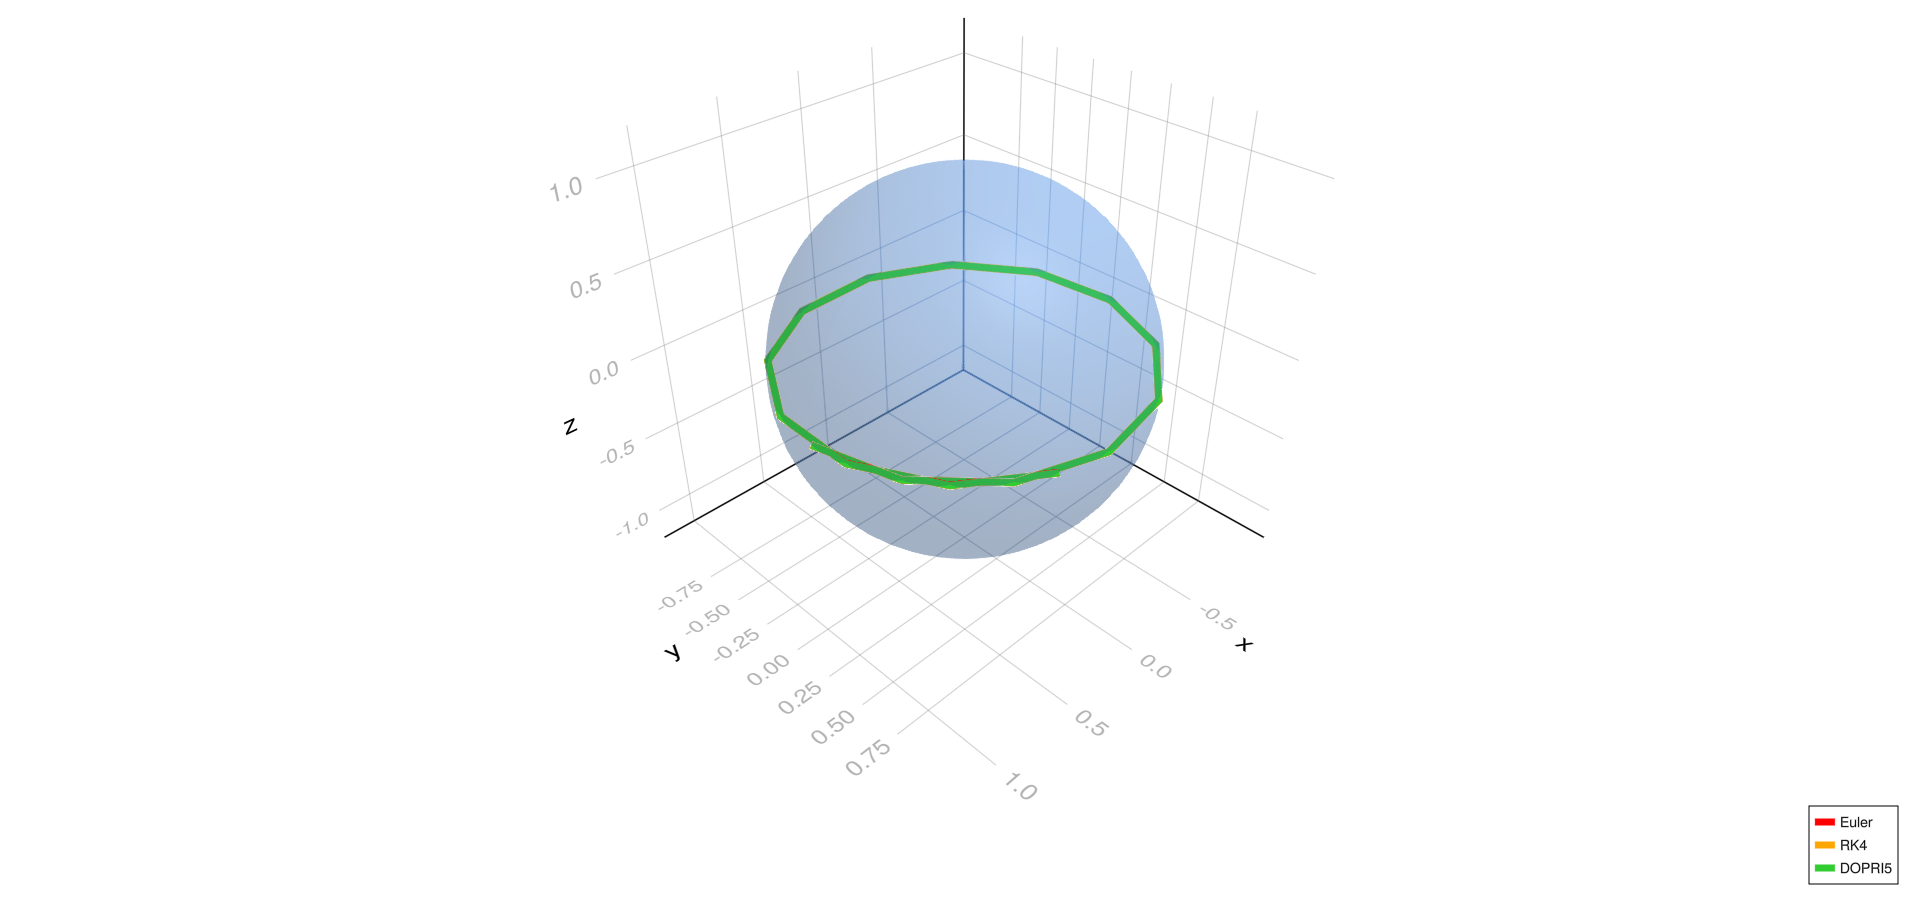
\includegraphics[width=\linewidth]{test.png}
			\caption{Equatorial geodesic, \(h=1.0\)}
		\end{subfigure}
		
		\vspace{3em}
		
		\begin{subfigure}{1\textwidth}
			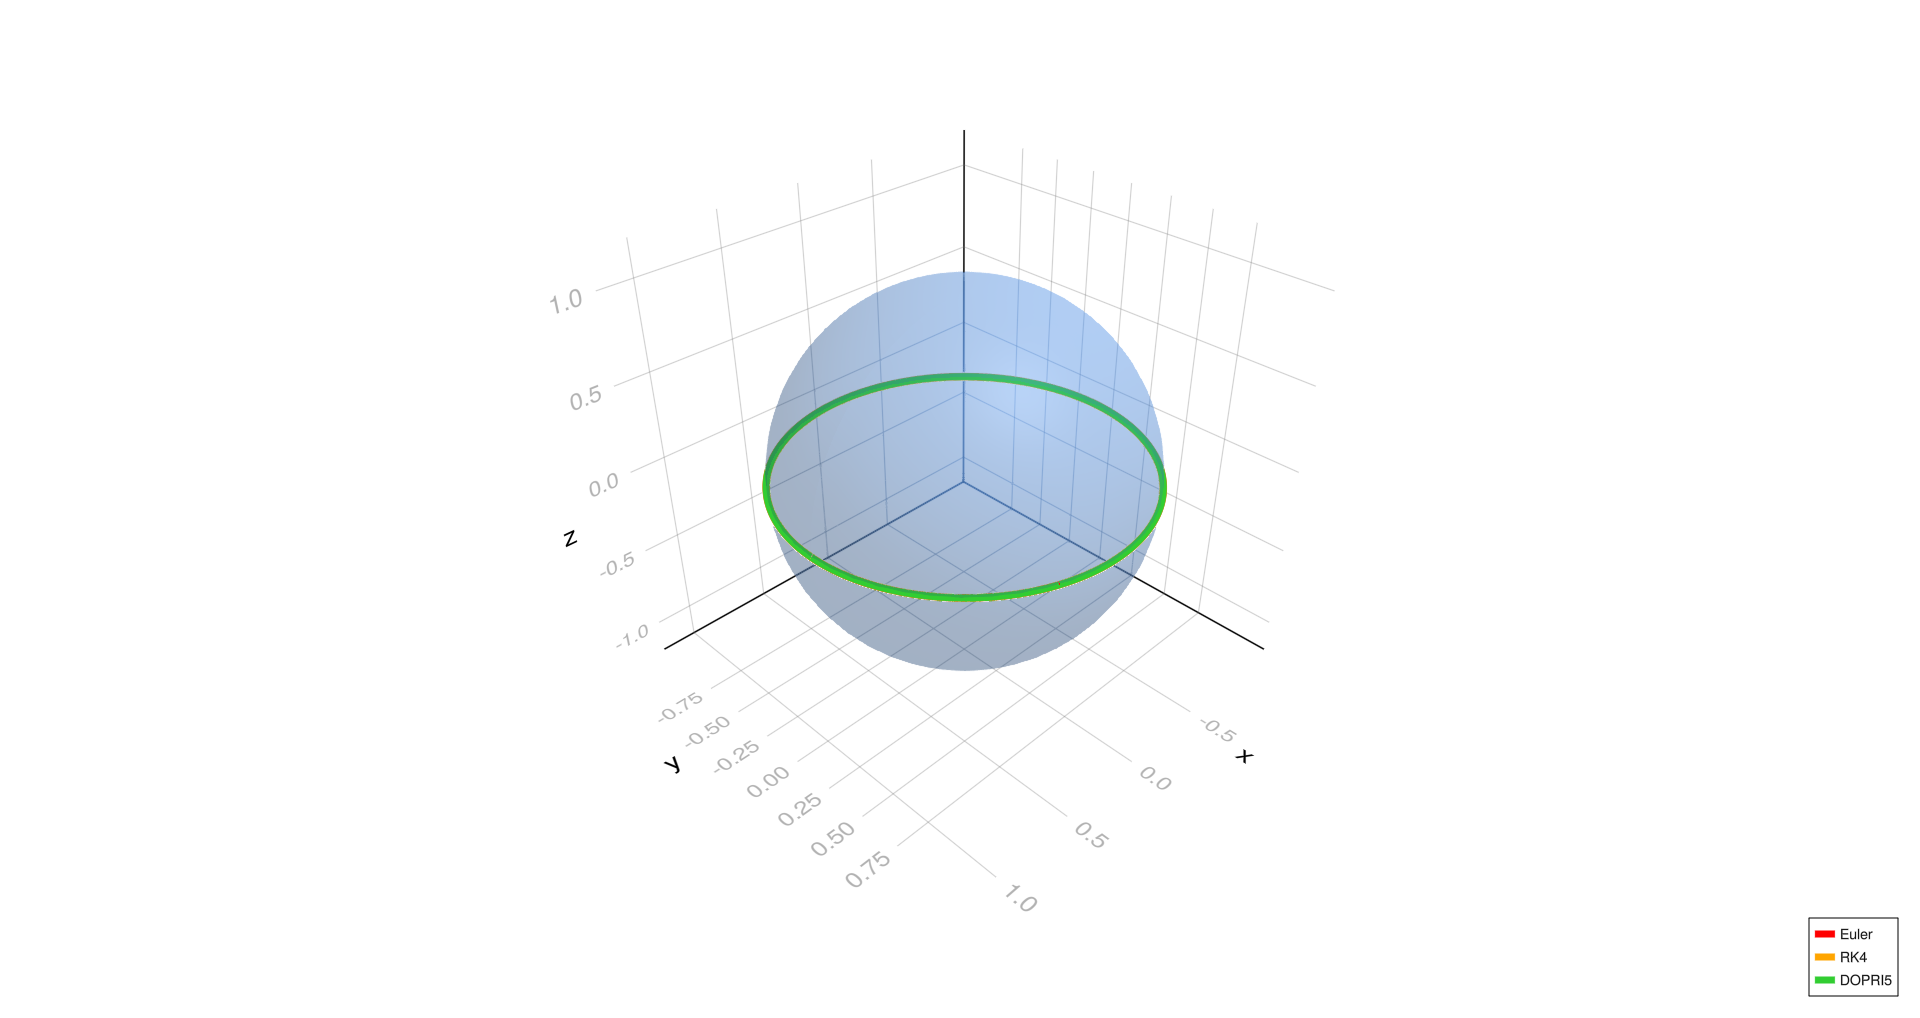
\includegraphics[width=\linewidth]{hor_eq_h01.png}
			\caption{Equatorial geodesic, \(h=0.01\)}
		\end{subfigure}
		
		\caption{Geodesics on the sphere.}
	\end{figure}
	
	\clearpage
	\begin{figure}[H]
		\centering
		\begin{subfigure}{1\textwidth}
			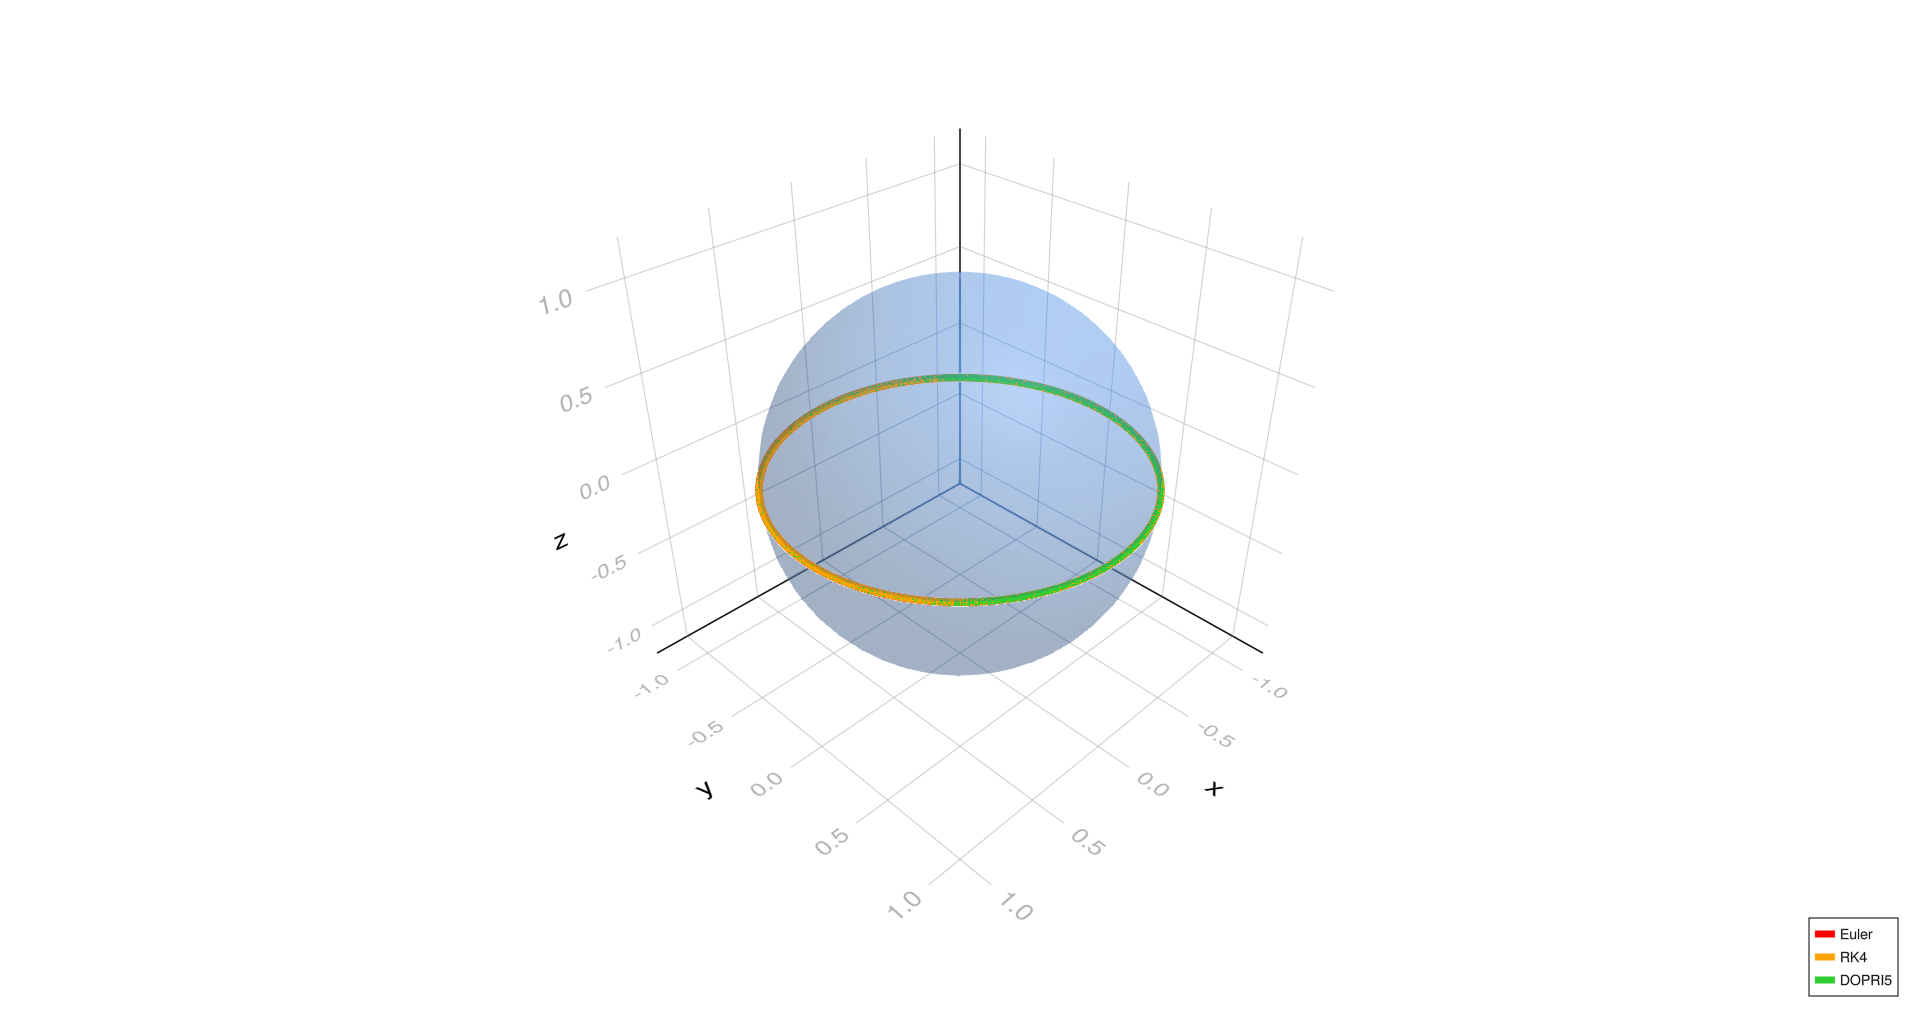
\includegraphics[width=\linewidth]{hor_eq_h0001.png}
			\caption{Equatorial geodesic, \(h=0.0001\)}
		\end{subfigure}
		
		\vspace{3em}
		
		\begin{subfigure}{1\textwidth}
			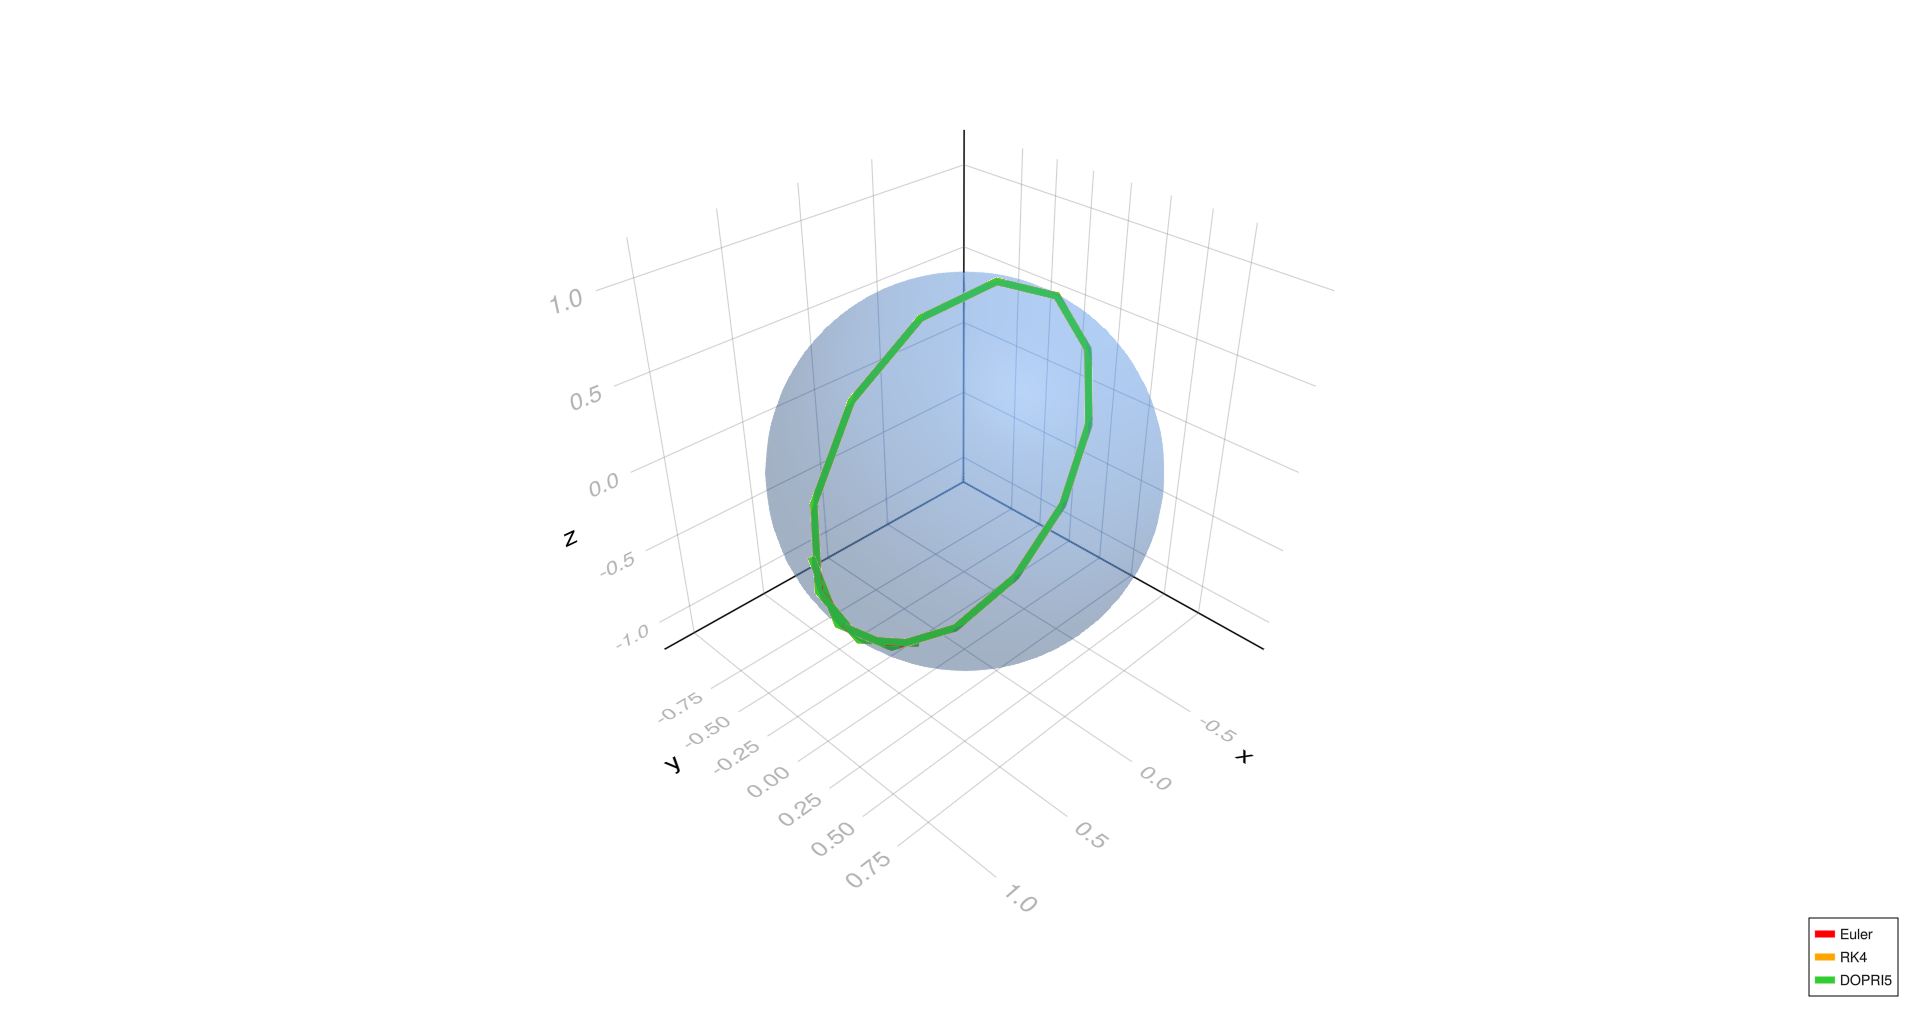
\includegraphics[width=\linewidth]{ver_eq_h1.png}
			\caption{Meridional geodesic, \(h=1.0\)}
		\end{subfigure}
		
		\caption{Geodesics on the sphere.}
	\end{figure}
	
	\clearpage
	\begin{figure}[H]
		\centering
		\begin{subfigure}{1\textwidth}
			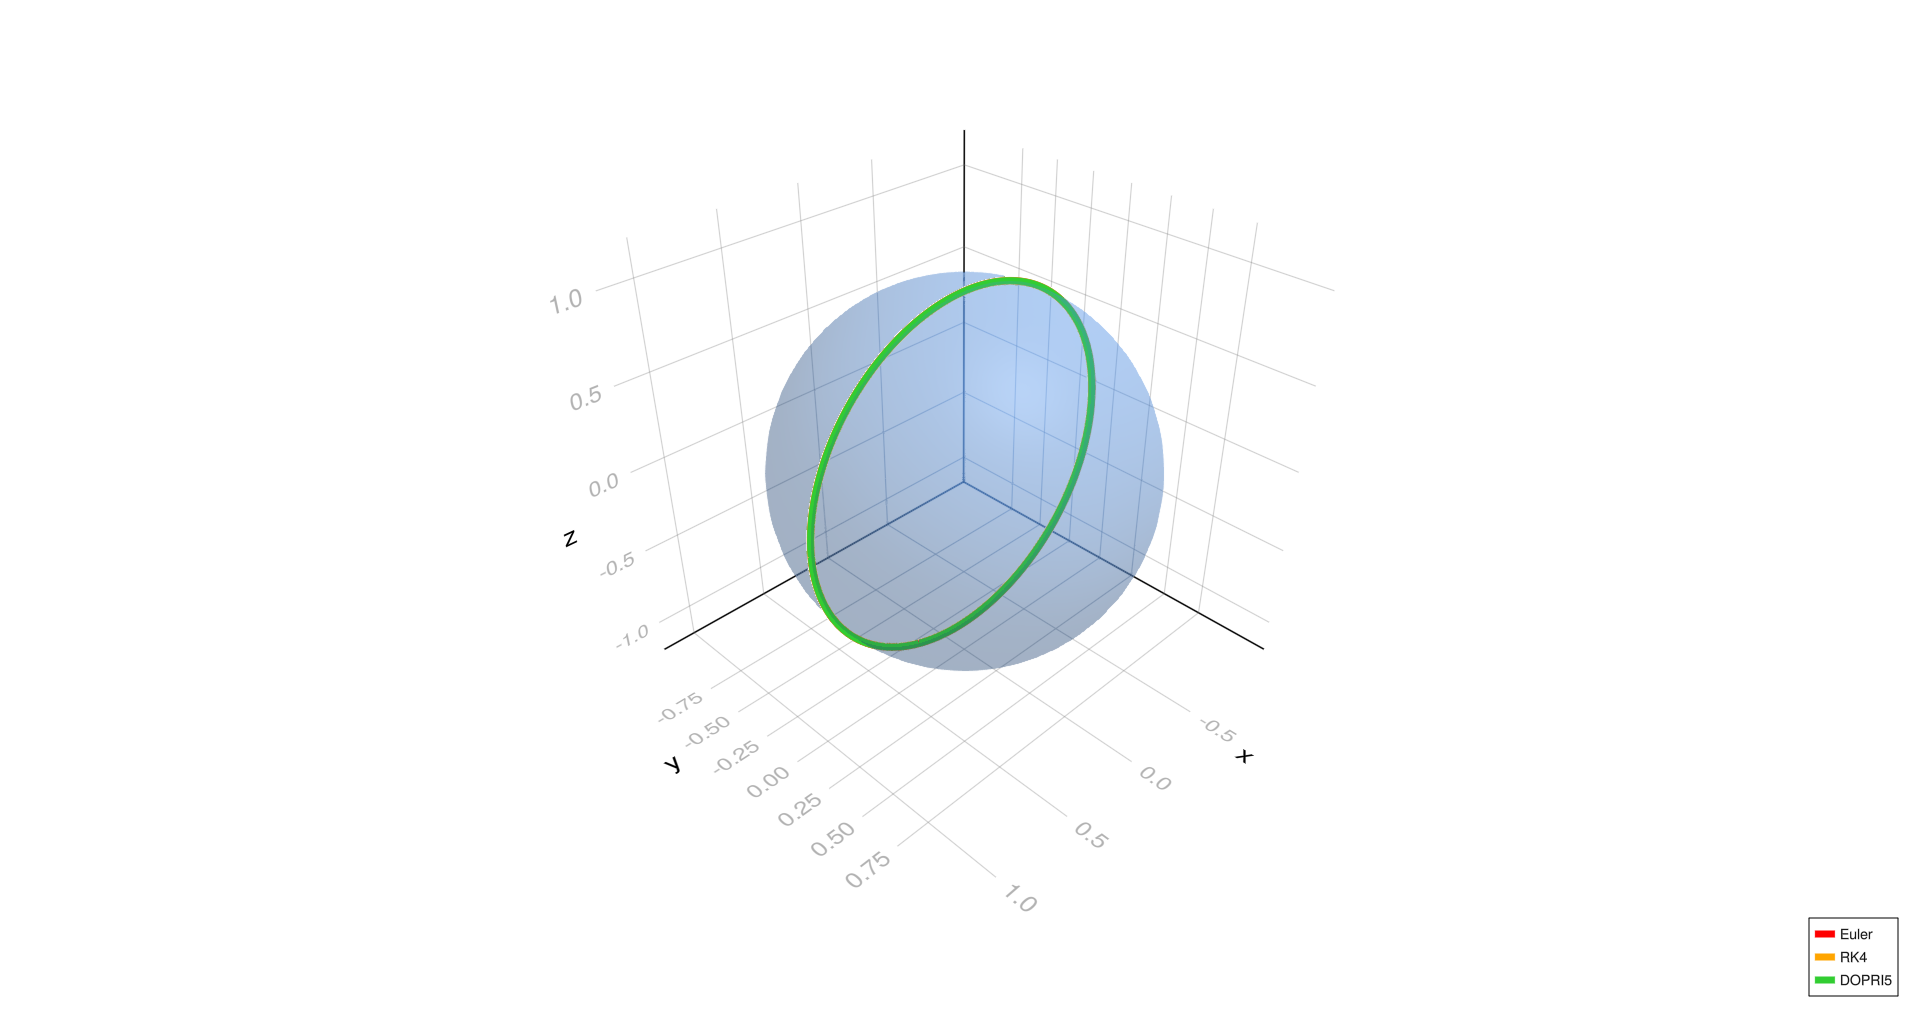
\includegraphics[width=\linewidth]{ver_eq_h01.png}
			\caption{Meridional geodesic, \(h=0.01\)}
		\end{subfigure}
		
		\vspace{3em}
		
		\begin{subfigure}{1\textwidth}
			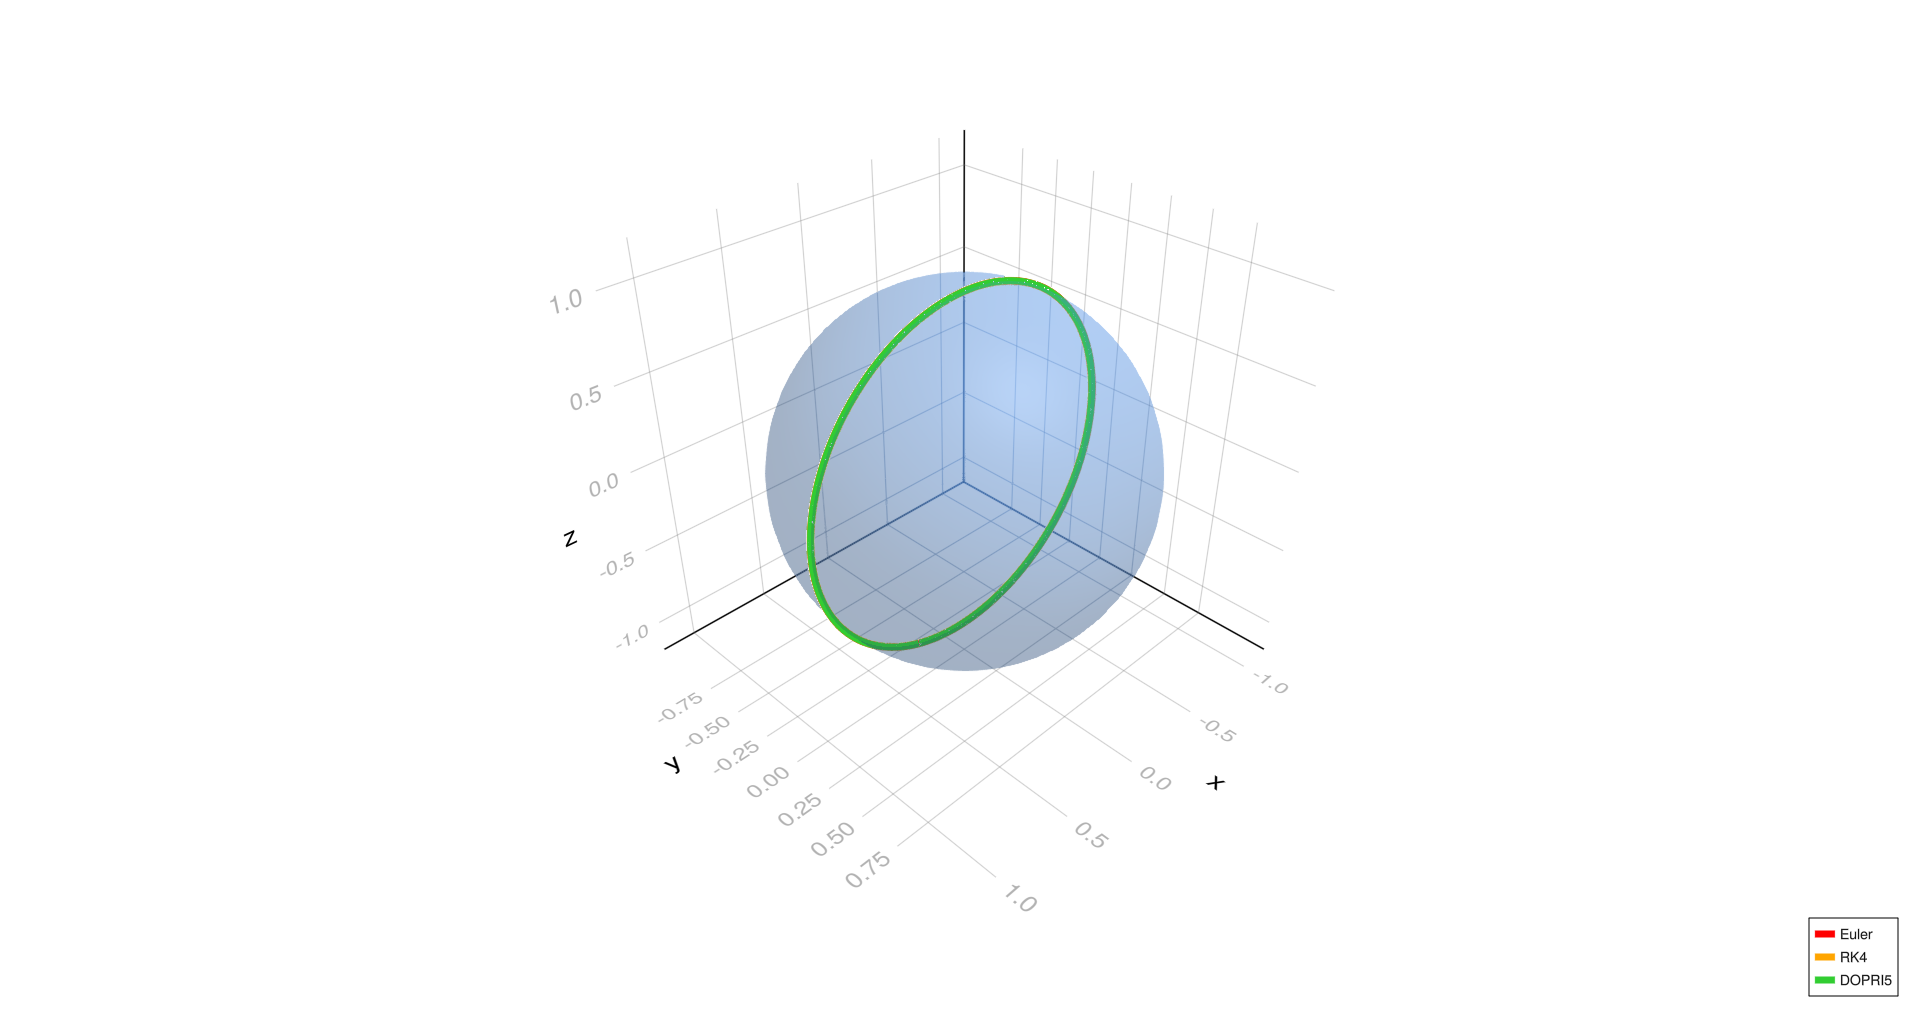
\includegraphics[width=\linewidth]{ver_eq_h0001.png}
			\caption{Meridional geodesic, \(h=0.0001\)}
		\end{subfigure}
		
		\caption{Geodesics on the sphere.}
	\end{figure}
	
	\clearpage
	\begin{figure}[H]
		\centering
		\begin{subfigure}{1\textwidth}
			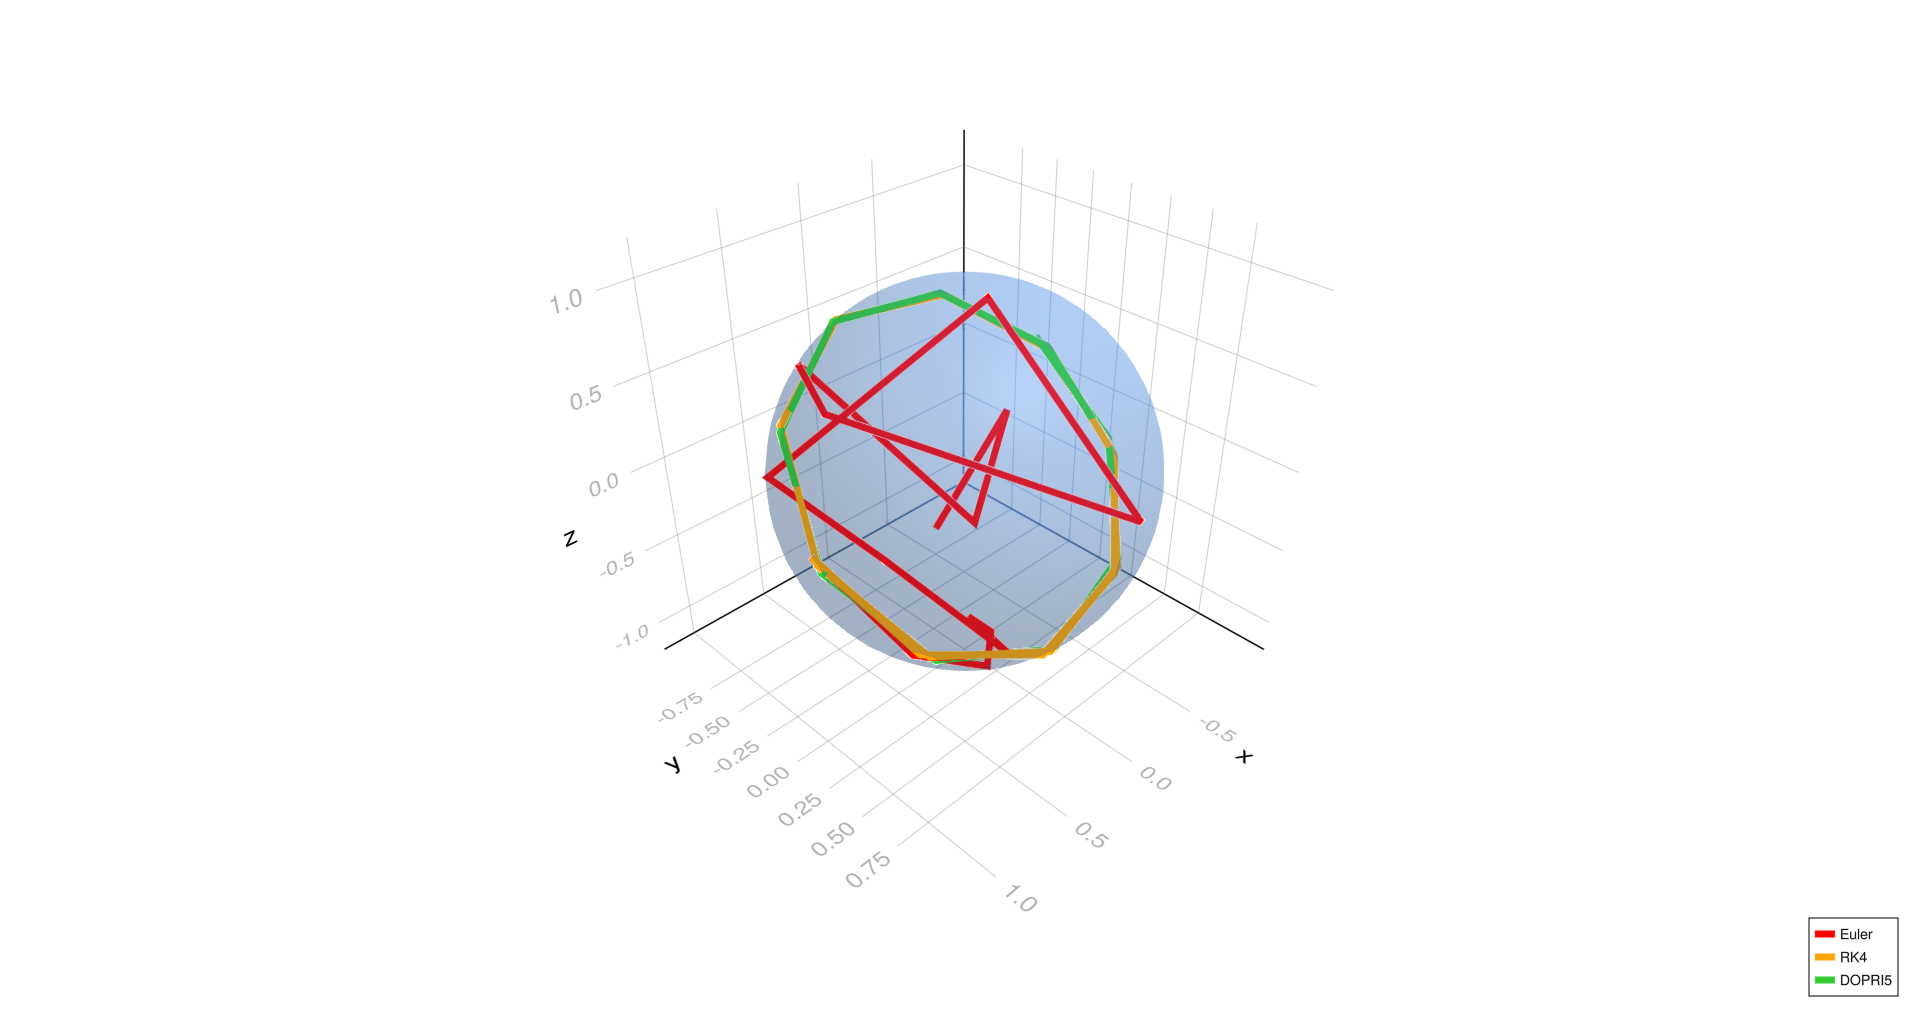
\includegraphics[width=\linewidth]{dia_h1.png}
			\caption{Diagonal geodesic, \(h=1.0\)}
		\end{subfigure}
		
		\vspace{3em}
		
		\begin{subfigure}{1\textwidth}
			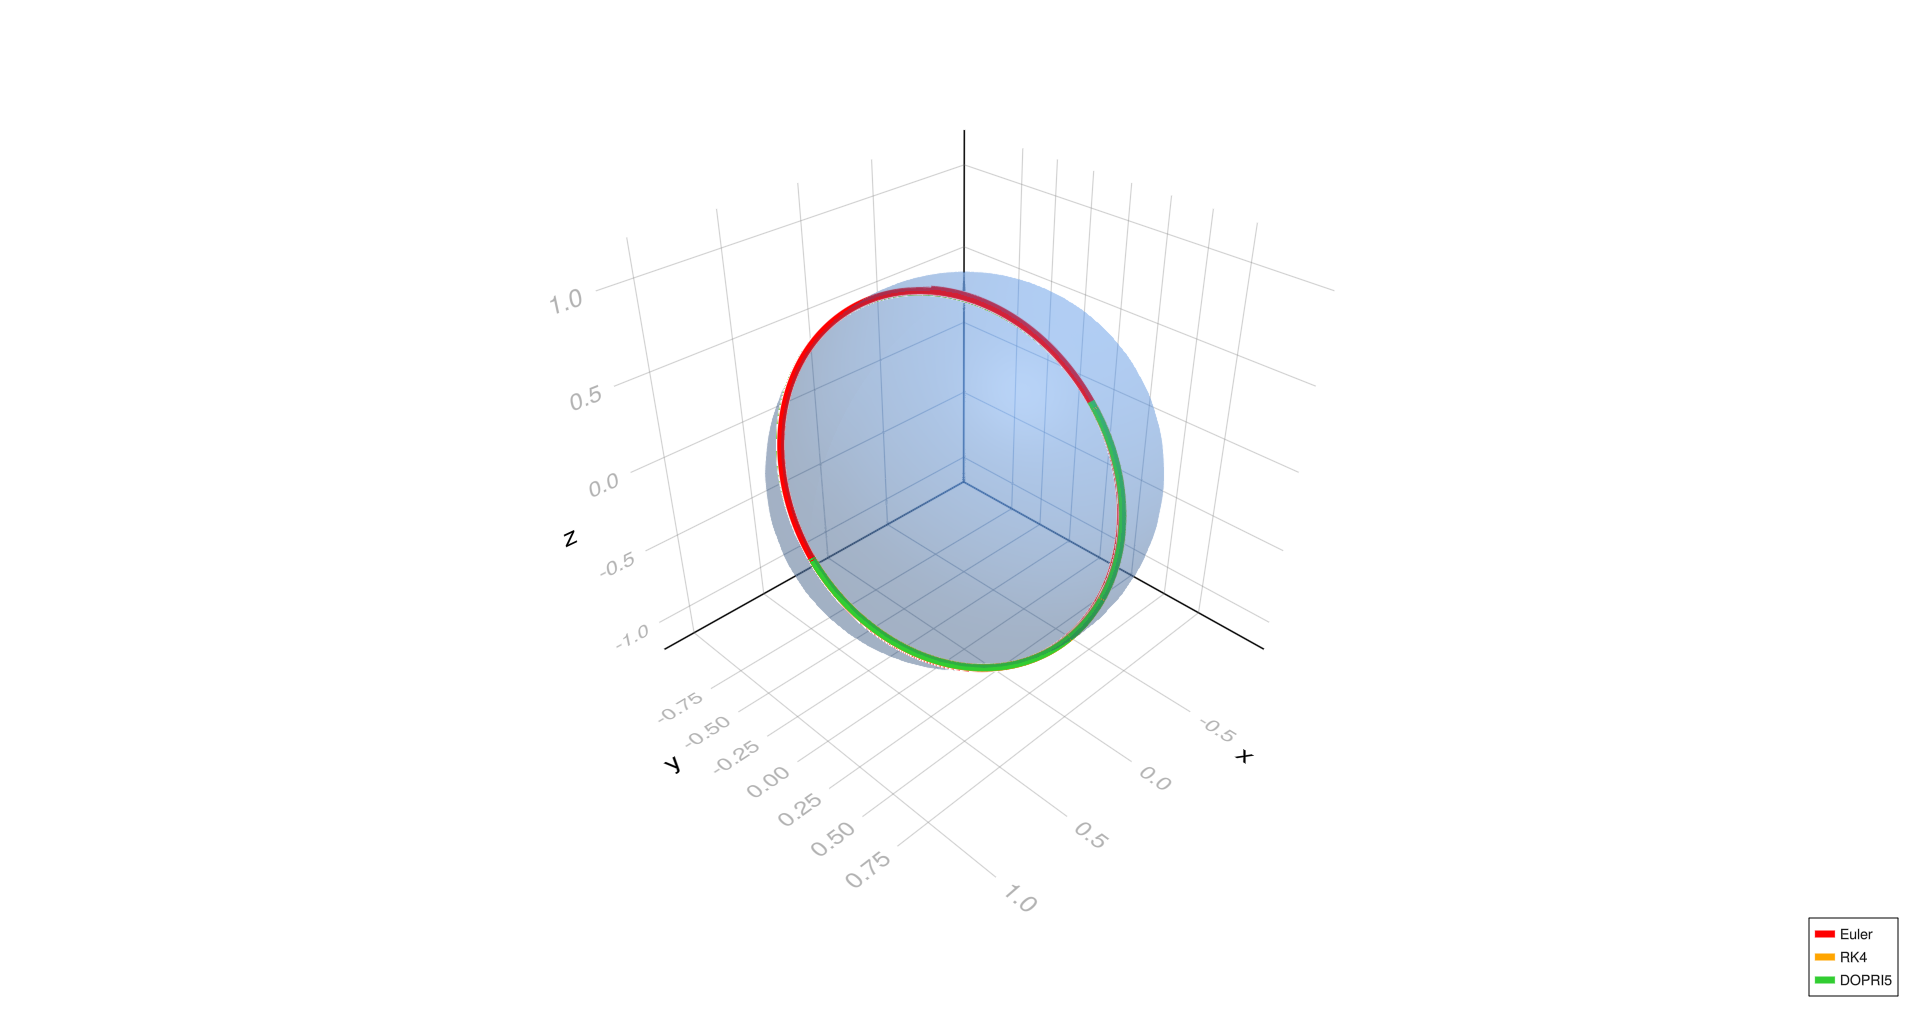
\includegraphics[width=\linewidth]{dia_h01.png}
			\caption{Diagonal geodesic, \(h=0.01\)}
		\end{subfigure}
		
		\caption{Geodesics on the sphere.}
	\end{figure}
	
	\clearpage
	\begin{figure}[H]
		\centering
		\begin{subfigure}{1\textwidth}
			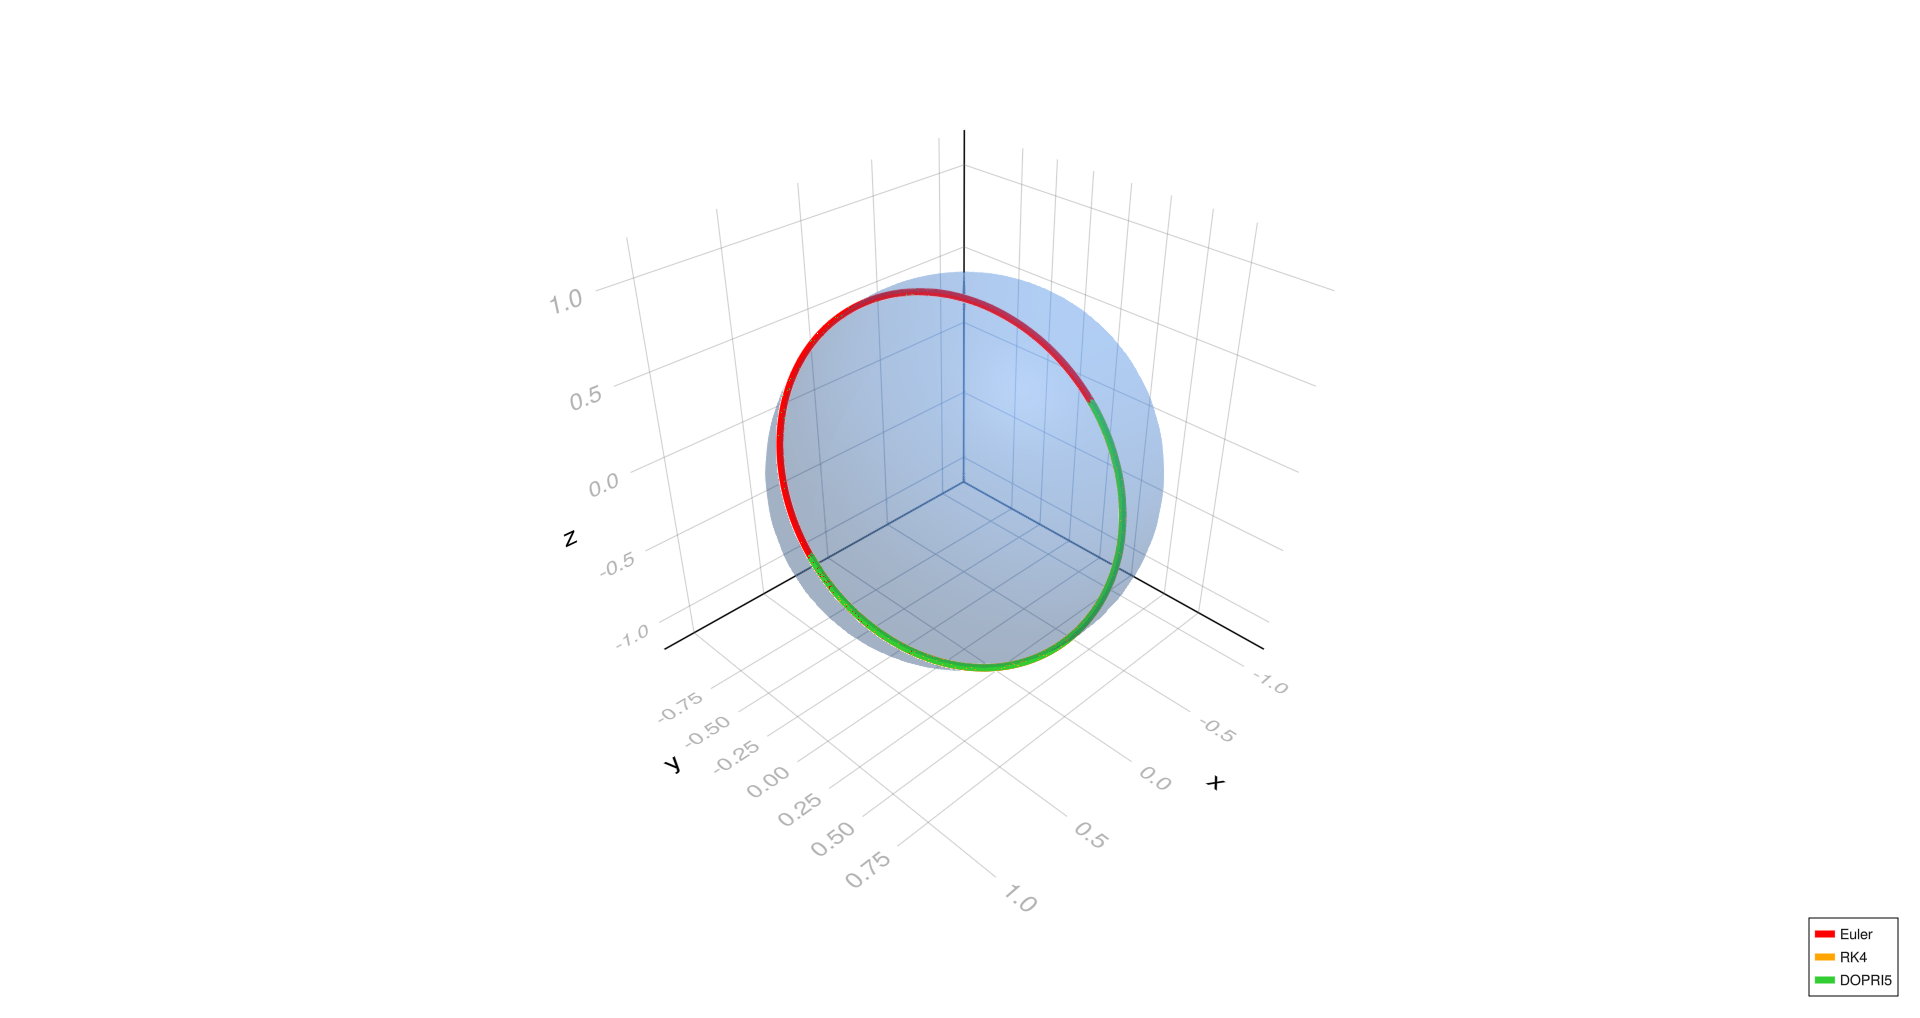
\includegraphics[width=\linewidth]{dia_h0001.png}
			\caption{Diagonal geodesic, \(h=0.0001\)}
		\end{subfigure}
		
		\vspace{3em}
		
		\begin{subfigure}{1\textwidth}
			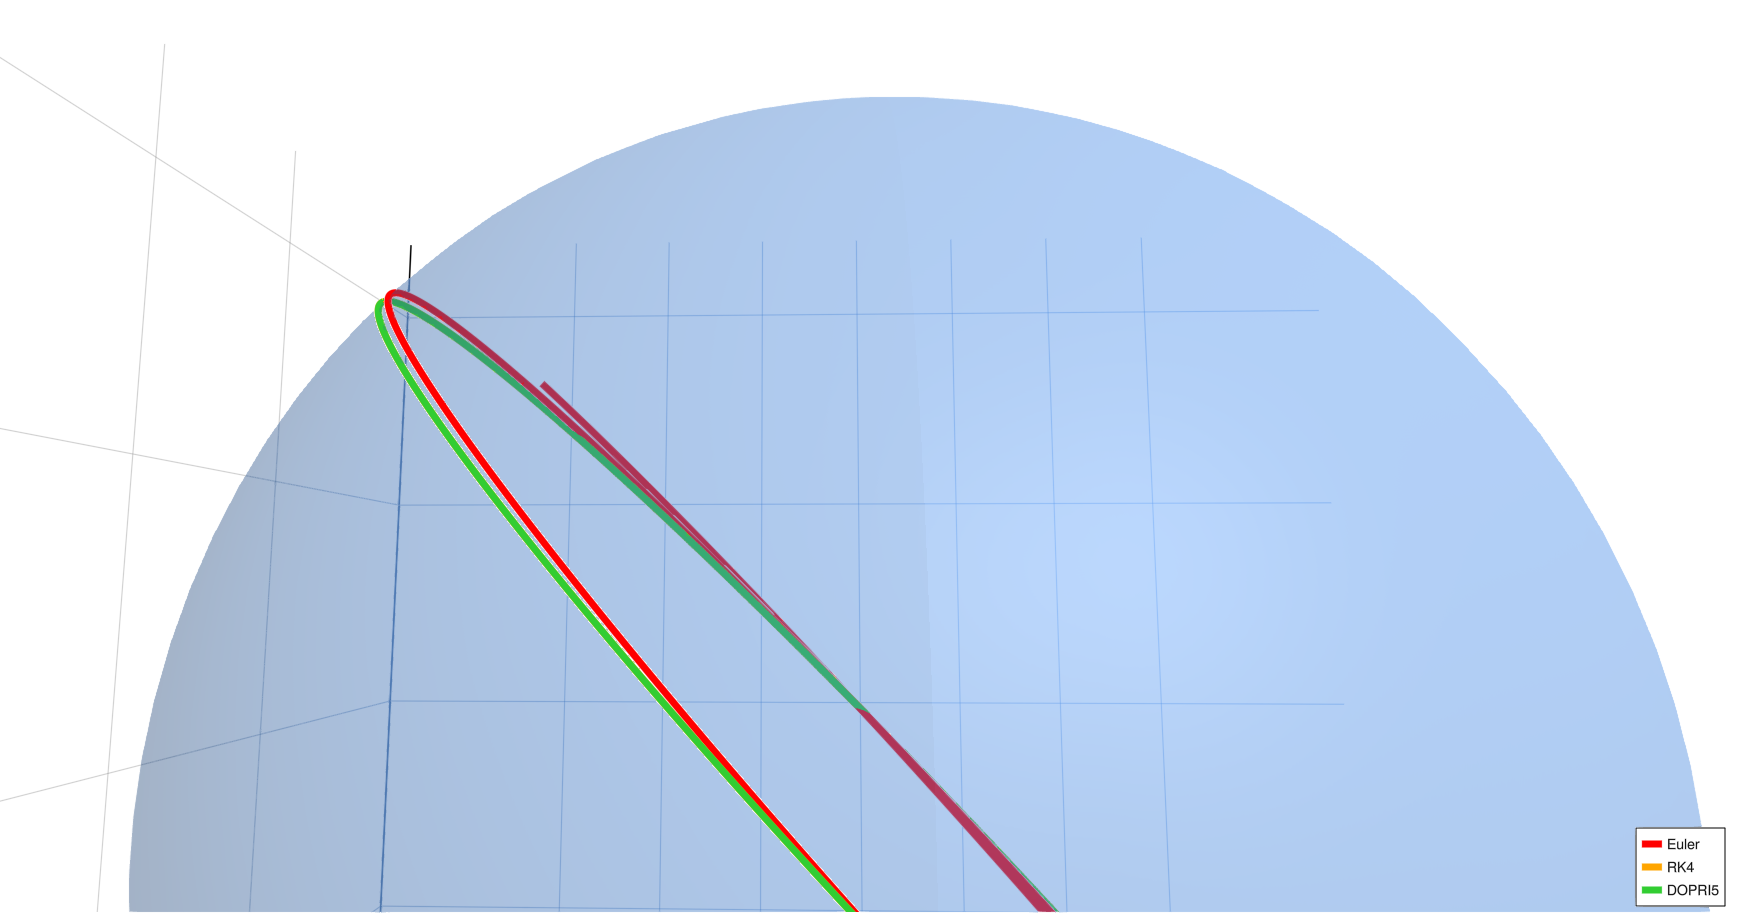
\includegraphics[width=\linewidth]{dia_h01_upclose.png}
			\caption{Diagonal geodesic, \(h=0.01\) (detailed view)}
		\end{subfigure}
		
		\caption{Geodesics on the sphere.}
	\end{figure}
	
	\clearpage
	\begin{figure}[H]
		\centering
		\begin{subfigure}{1\textwidth}
			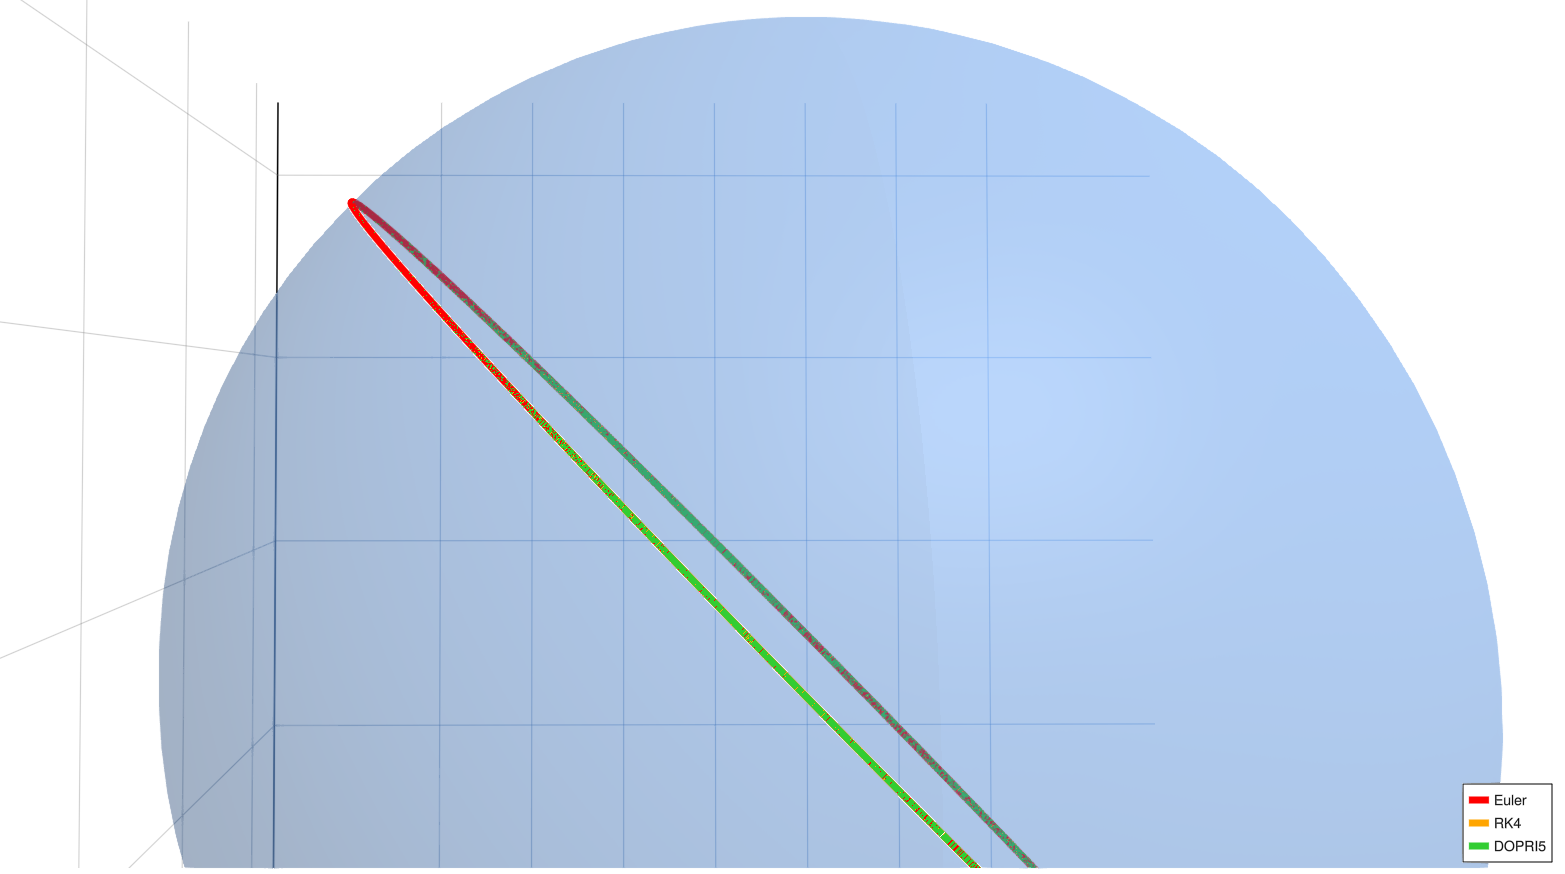
\includegraphics[width=\linewidth]{dia_h0001_upclose.png}
			\caption{Diagonal geodesic, \(h=0.0001\) (detailed view)}
		\end{subfigure}
		
		\caption{Geodesics on the sphere.}
	\end{figure}

	\newpage
		\subsubsection{Empirical Observations}
	
	\begin{itemize}
		\item The \textit{equatorial} and \textit{meridional geodesic} cases show excellent agreement among all three methods (Euler, RK4, DOPRI5) at all step sizes, indicating stable geodesics.
		\item For the \textit{diagonal geodesic} case, Euler's method deviates noticeably at \(h=1.0\) and slightly at \(h=0.01\), while RK4 and DOPRI5 remain well aligned.
		\item At the finest step size \(h=0.0001\), all methods align closely even in the diagonal case, confirming that reducing step size improves Euler's accuracy.
	\end{itemize}
	\subsubsection{Summary Table of Empirical Stability}
	
	\begin{table}[H]
		\centering
		\begin{tabular}{lccc}
			\toprule
			\textbf{Initial Condition} & \textbf{Step Size} & \textbf{Euler Accuracy} & \textbf{RK4 / DOPRI5 Accuracy} \\
			\midrule
			Equatorial geodesic & 1.0 & Stable & Stable \\
			& 0.01 & Stable & Stable \\
			& 0.0001 & Stable & Stable \\
			\midrule
			Meridional geodesic & 1.0 & Stable & Stable \\
			& 0.01 & Stable & Stable \\
			& 0.0001 & Stable & Stable \\
			\midrule
			Diagonal geodesic & 1.0 & Large deviation & Stable \\
			& 0.01 & Minor deviation & Stable \\
			& 0.0001 & Stable & Stable \\
			\bottomrule
		\end{tabular}
		\caption{Empirical assessment of stability and accuracy of numerical methods for geodesics on the sphere.}
	\end{table}
	\newpage
	
	\subsection{Torus}
	
	\subsubsection{Initial Conditions}
	
	We test six distinct initial conditions representing geodesics on the torus:
	
	\begin{itemize}
		\item \textbf{Inner equator:} \(Y_0 = [\pi, 0.0, 0.0, 1.0]\)
		\item \textbf{Outer equator:} \(Y_0 = [0.0, 0.0, 0.0, 1.0]\)
		\item \textbf{Four turns:} \(Y_0 = [0.0, 1.0, 0.0, 0.1]\)
		\item \textbf{Complex spiral:} \(Y_0 = [0.0, 0.73, 0.0, 0.1]\)
		\item \textbf{Six turns:} \(Y_0 = [0.0, 0.69, 0.0, 0.05]\)
		\item \textbf{Triangle:} \(Y_0 = [0.0, 0.485, 0.0, 0.1]\)
	\end{itemize}
	
	\clearpage
	\begin{figure}[H]
		\centering
		\begin{subfigure}{1\textwidth}
			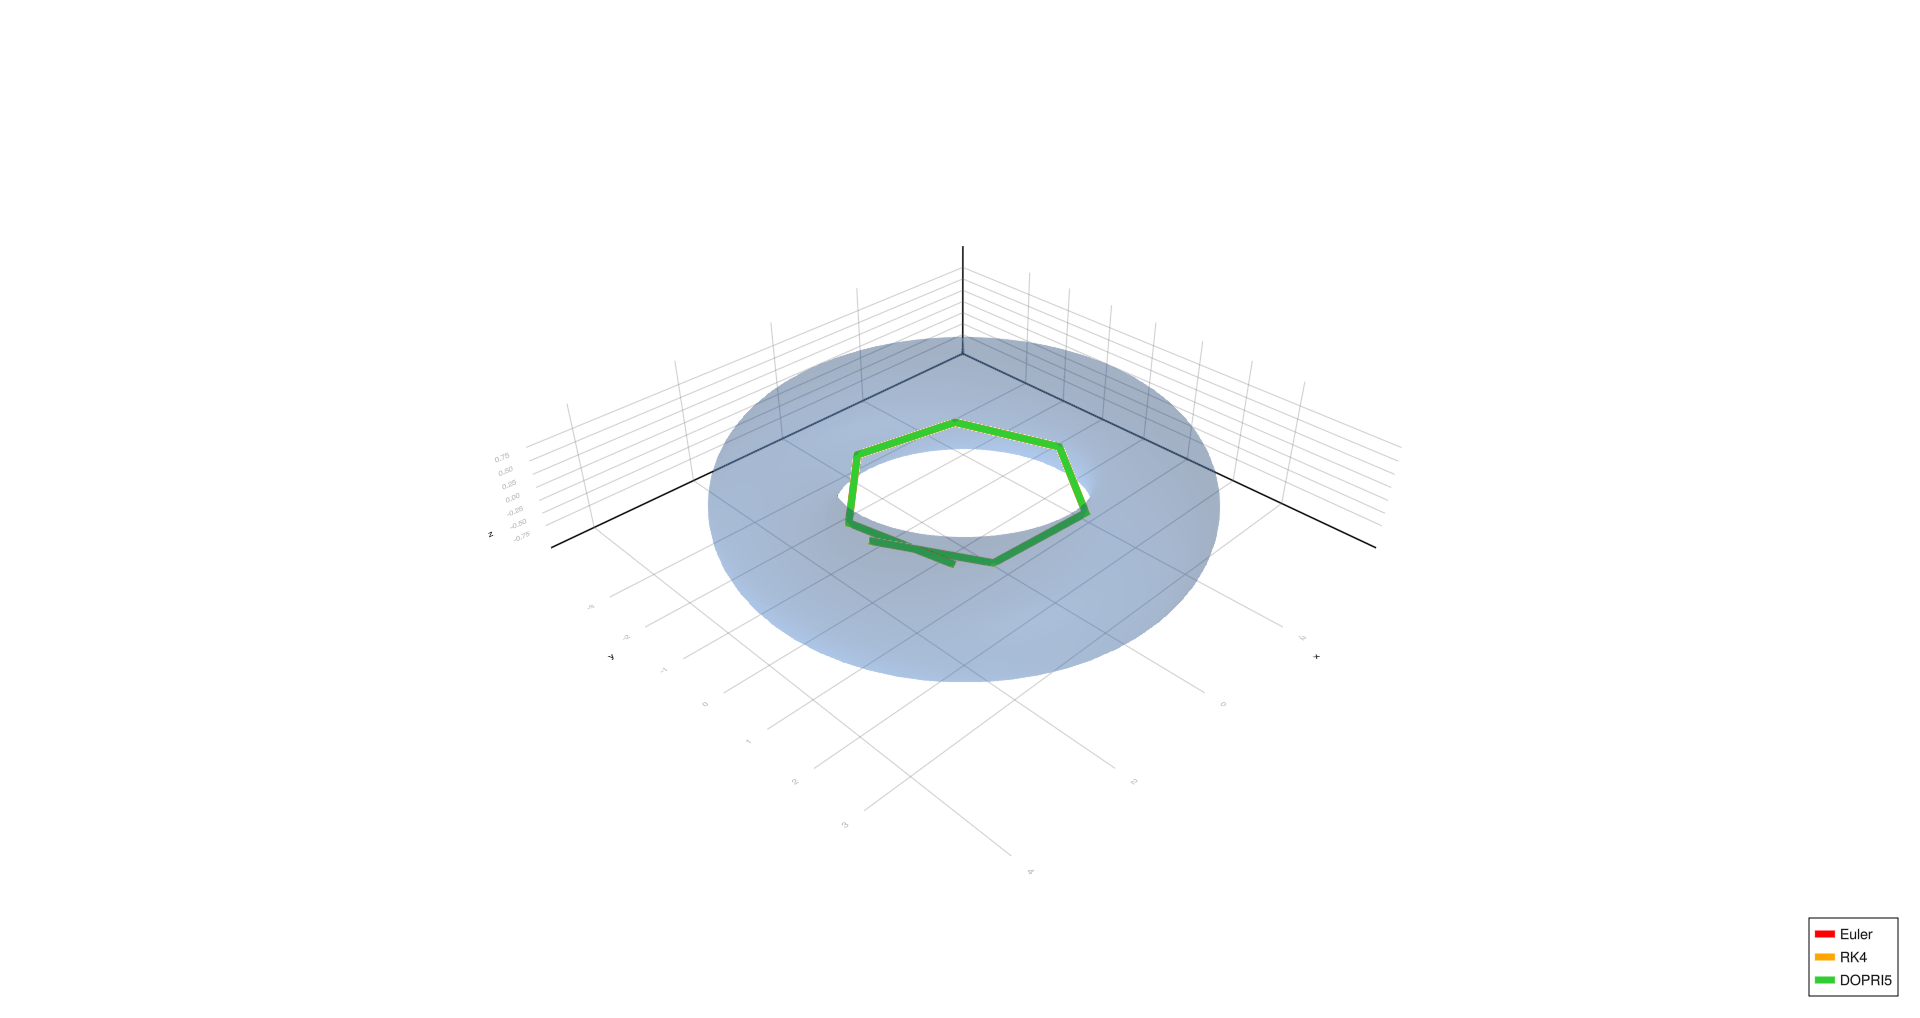
\includegraphics[width=\linewidth]{in_eq_h1.png}
			\caption{Inner equator, \(h=1.0\)}
		\end{subfigure}
		
		\vspace{3em}
		
		\begin{subfigure}{1\textwidth}
			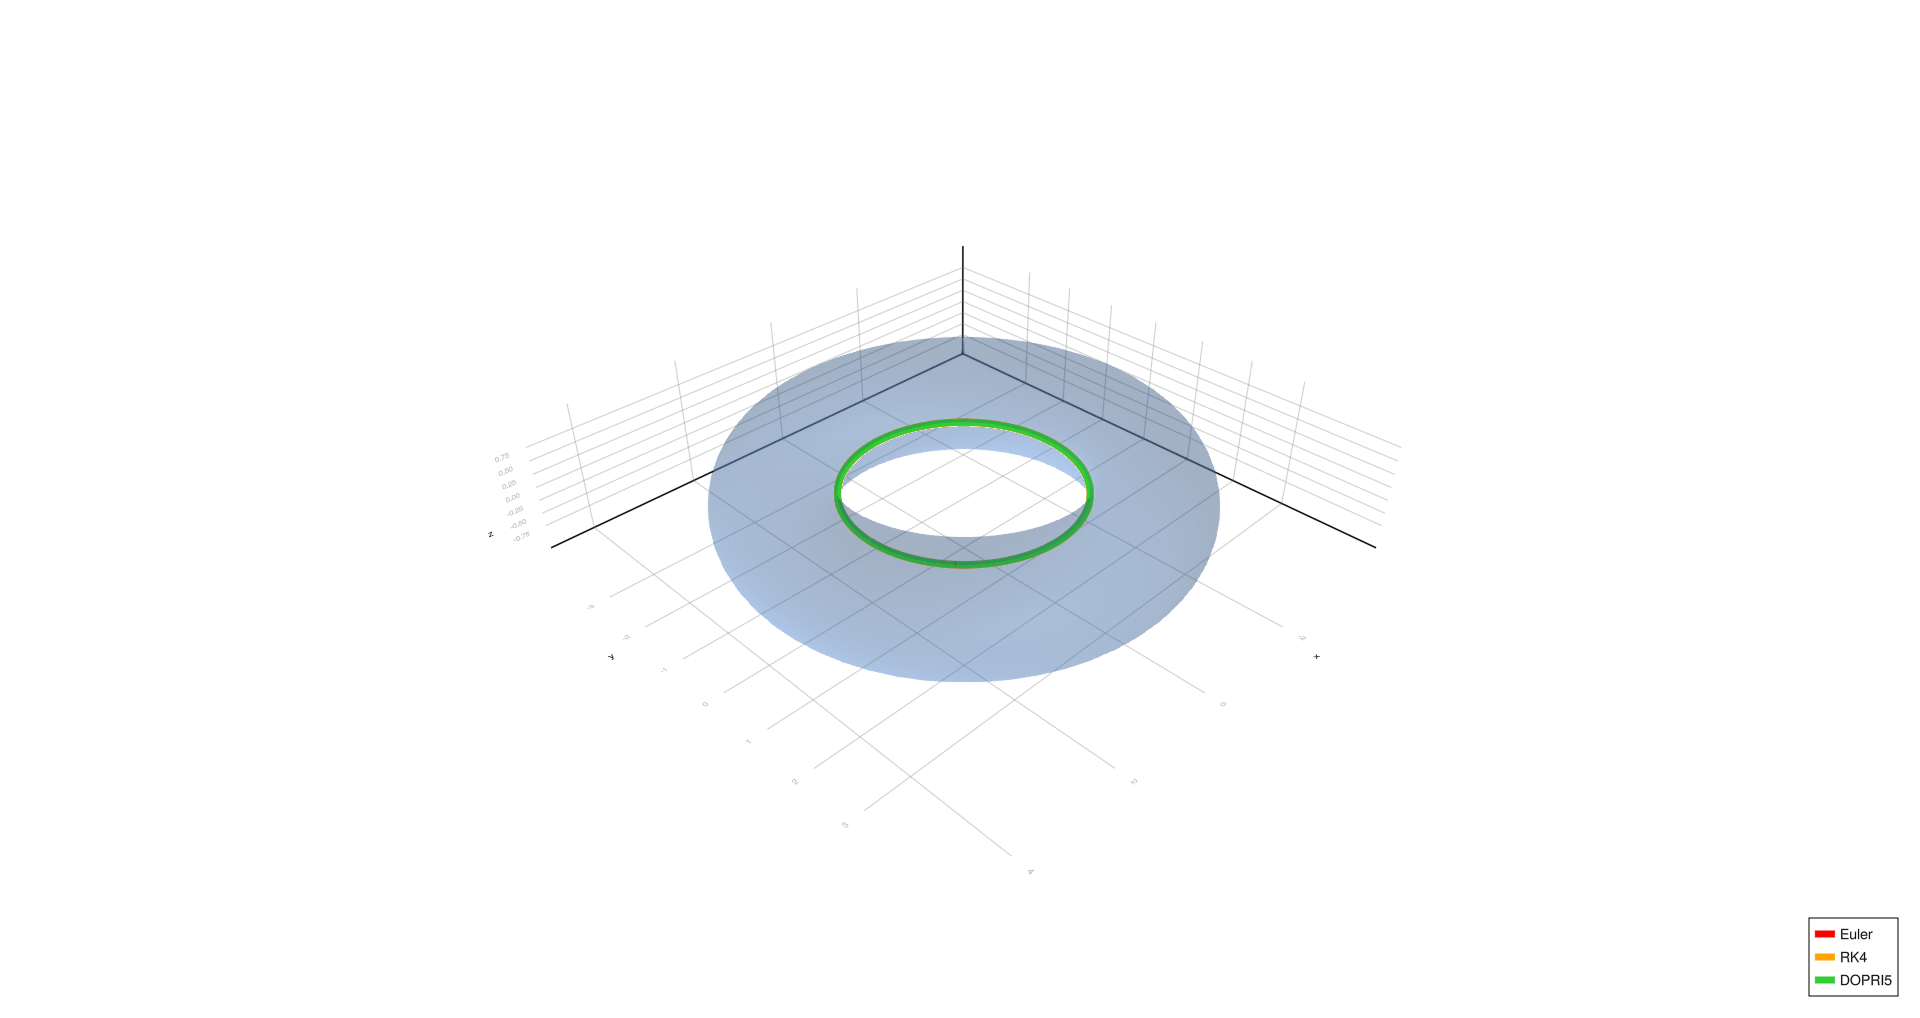
\includegraphics[width=\linewidth]{in_eq_h01.png}
			\caption{Inner equator, \(h=0.01\)}
		\end{subfigure}
		
		\caption{Torus geodesics}
	\end{figure}
	
	\clearpage
	\begin{figure}[H]
		\centering
		\begin{subfigure}{1\textwidth}
			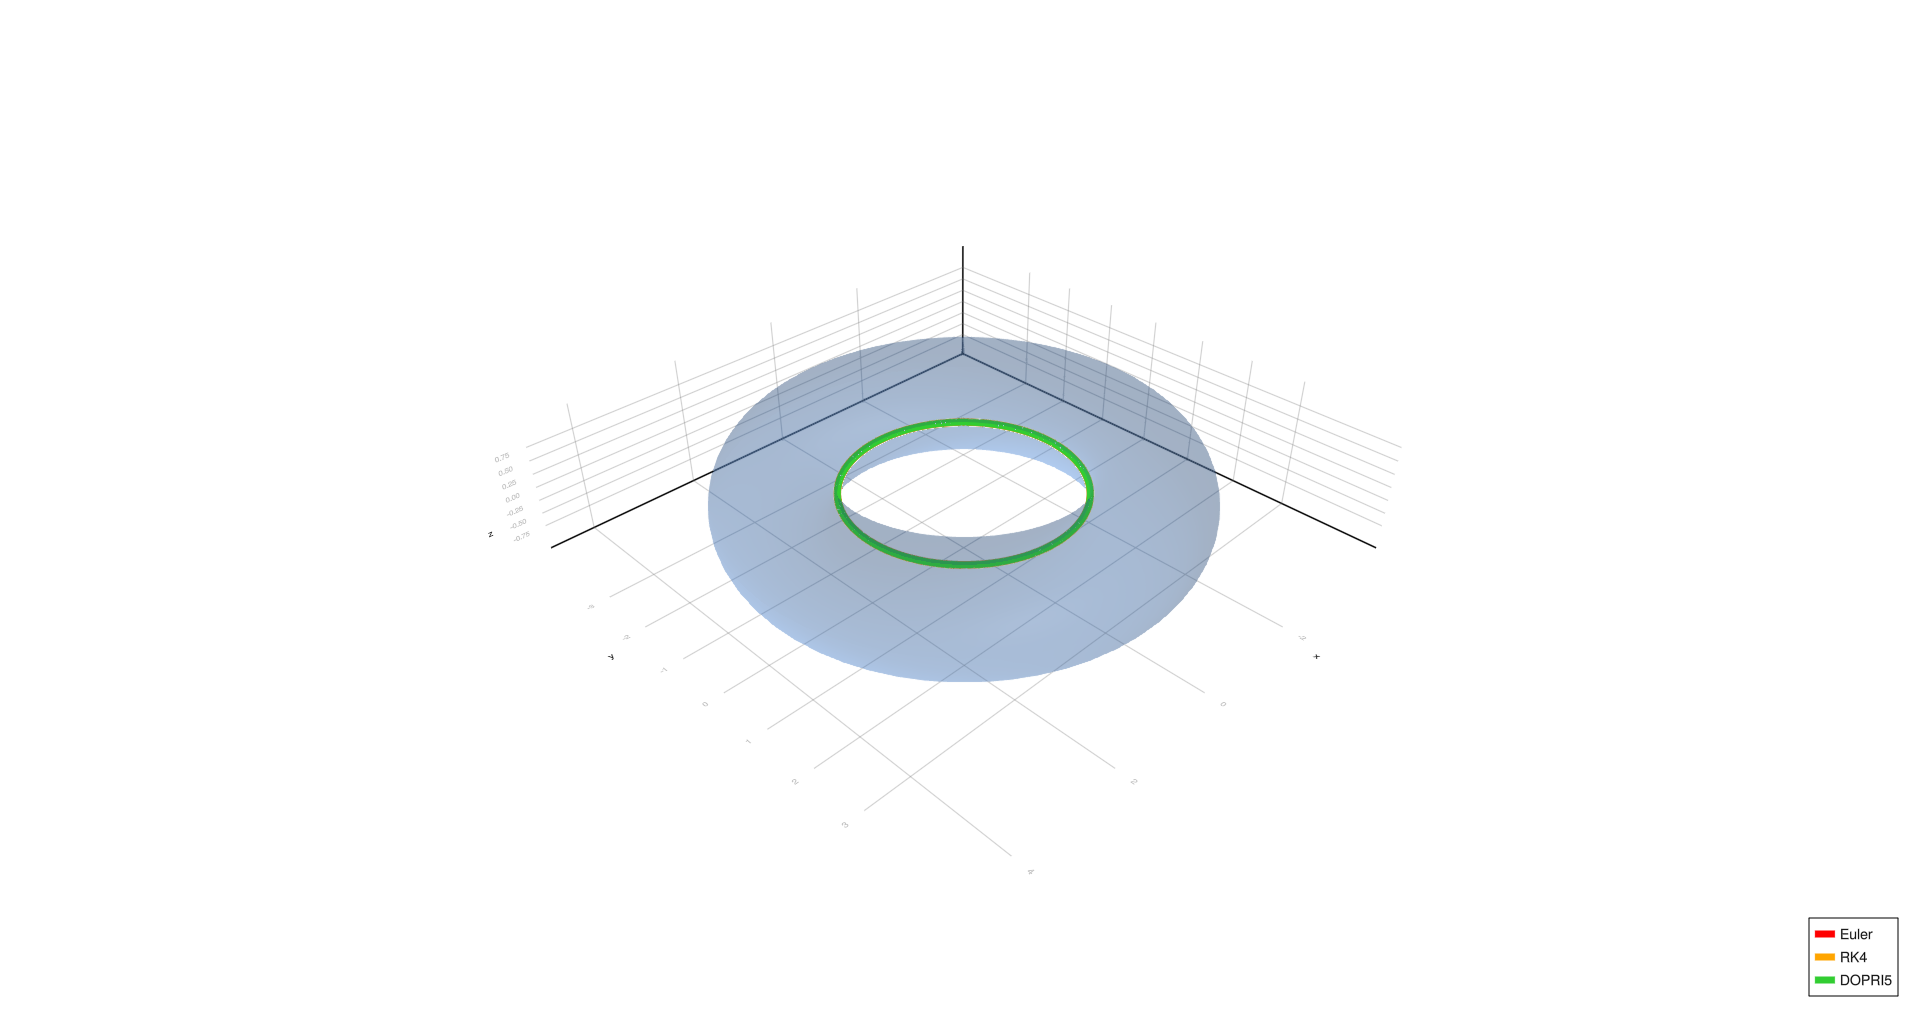
\includegraphics[width=\linewidth]{in_eq_h0001.png}
			\caption{Inner equator, \(h=0.0001\)}
		\end{subfigure}
		
		\vspace{3em}
		
		\begin{subfigure}{1\textwidth}
			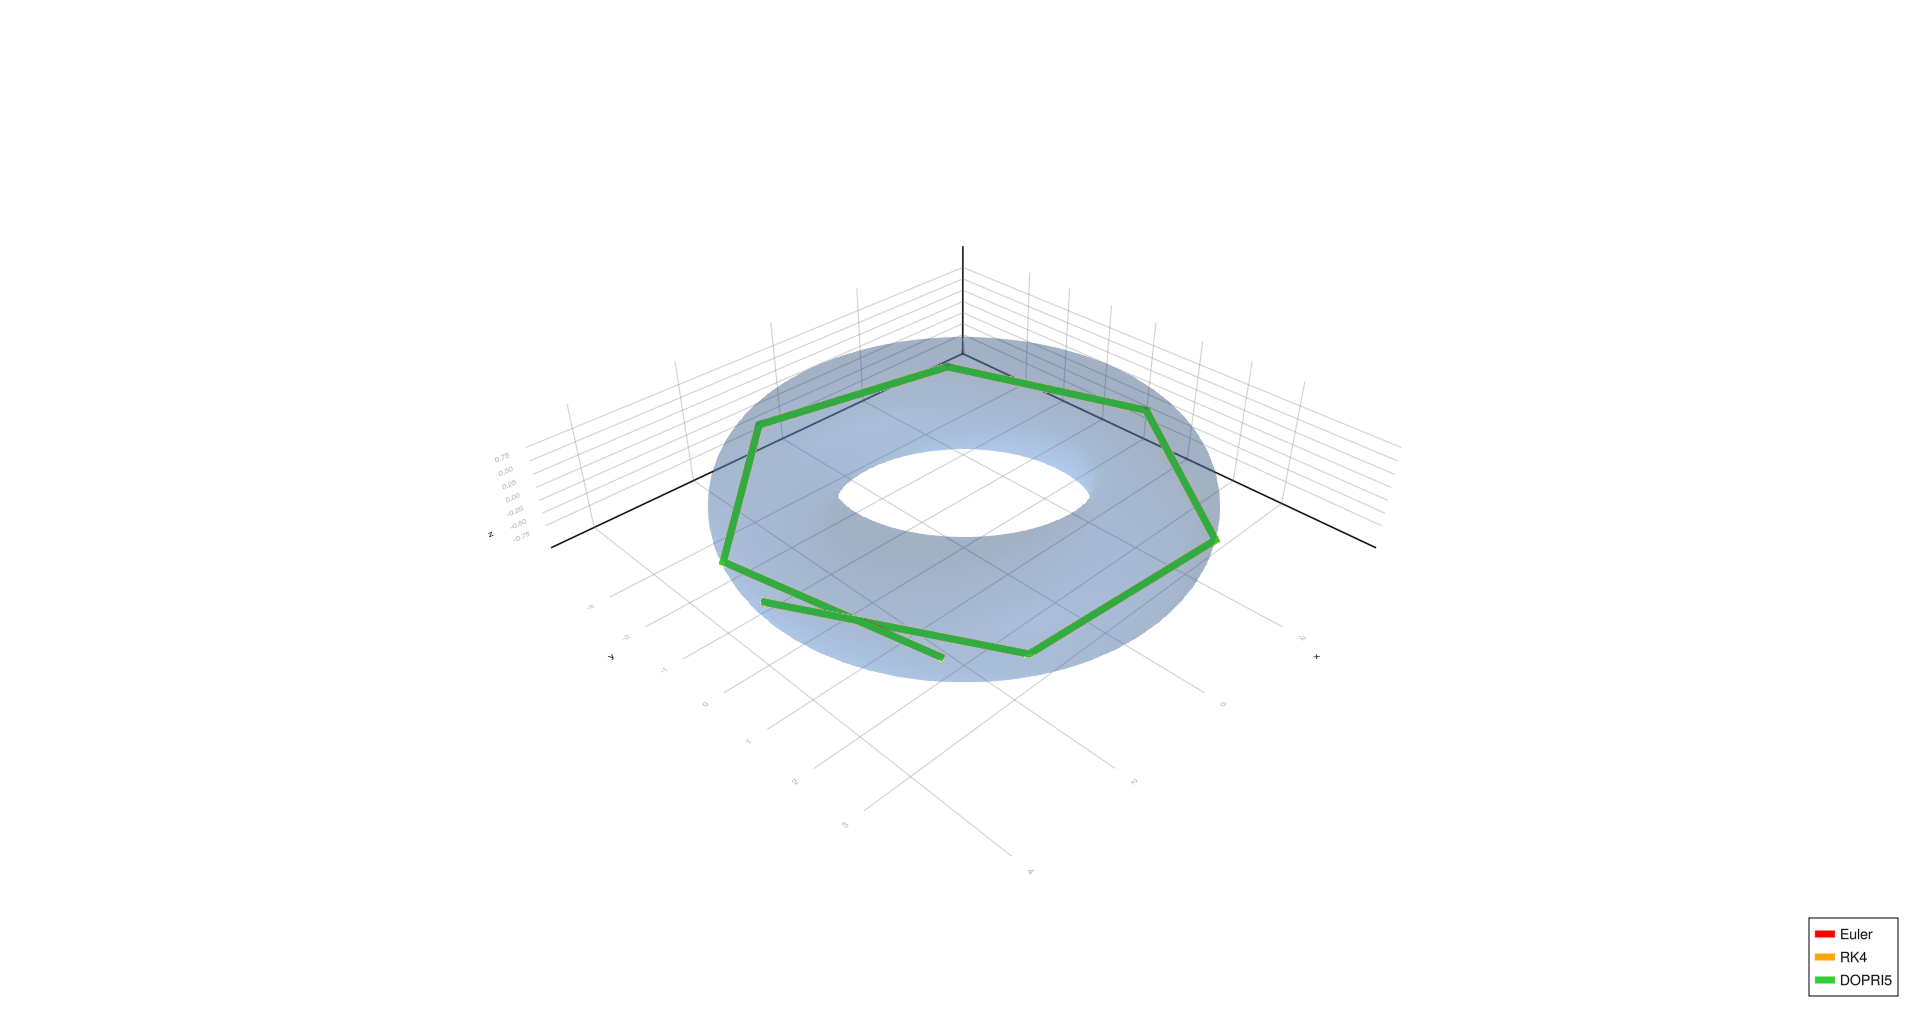
\includegraphics[width=\linewidth]{ou_eq_h1.png}
			\caption{Outer equator, \(h=1.0\)}
		\end{subfigure}
		
		\caption{Torus geodesics}
	\end{figure}
	
	\clearpage
	\begin{figure}[H]
		\centering
		\begin{subfigure}{1\textwidth}
			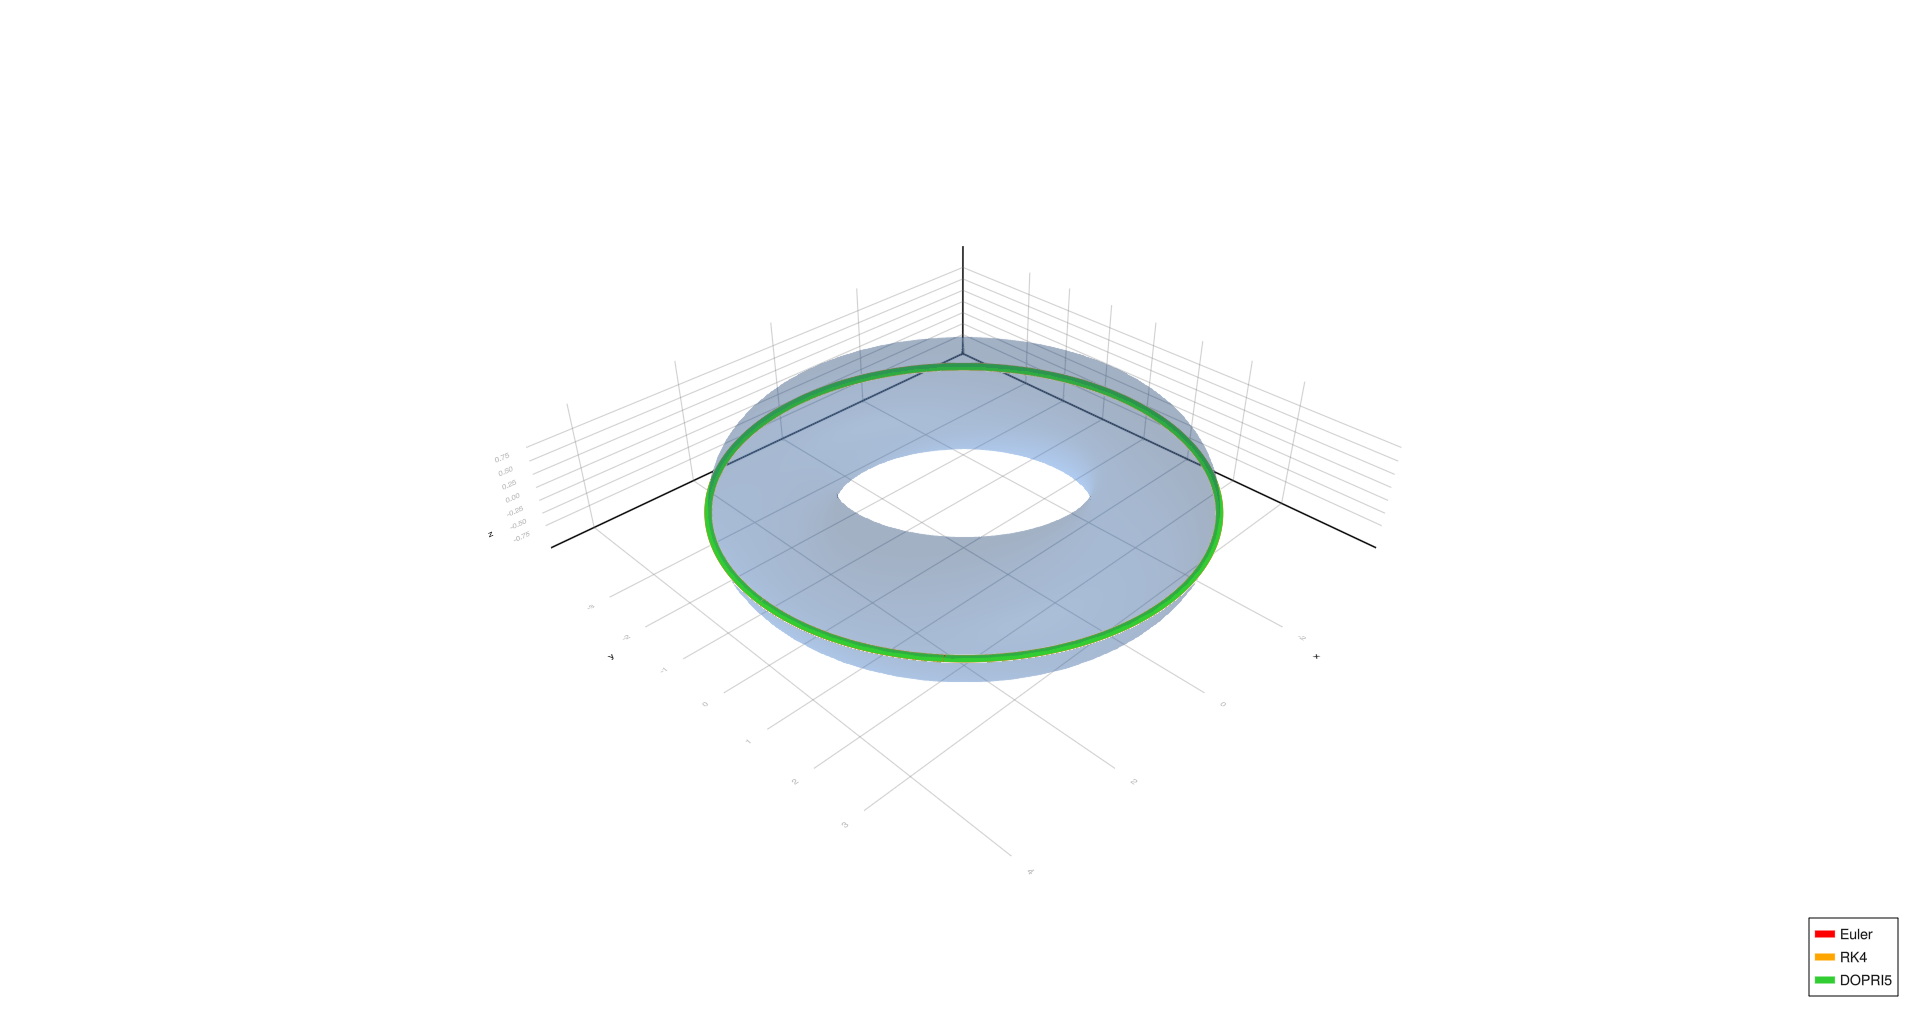
\includegraphics[width=\linewidth]{ou_eq_h01.png}
			\caption{Outer equator, \(h=0.01\)}
		\end{subfigure}
		
		\vspace{3em}
		
		\begin{subfigure}{1\textwidth}
			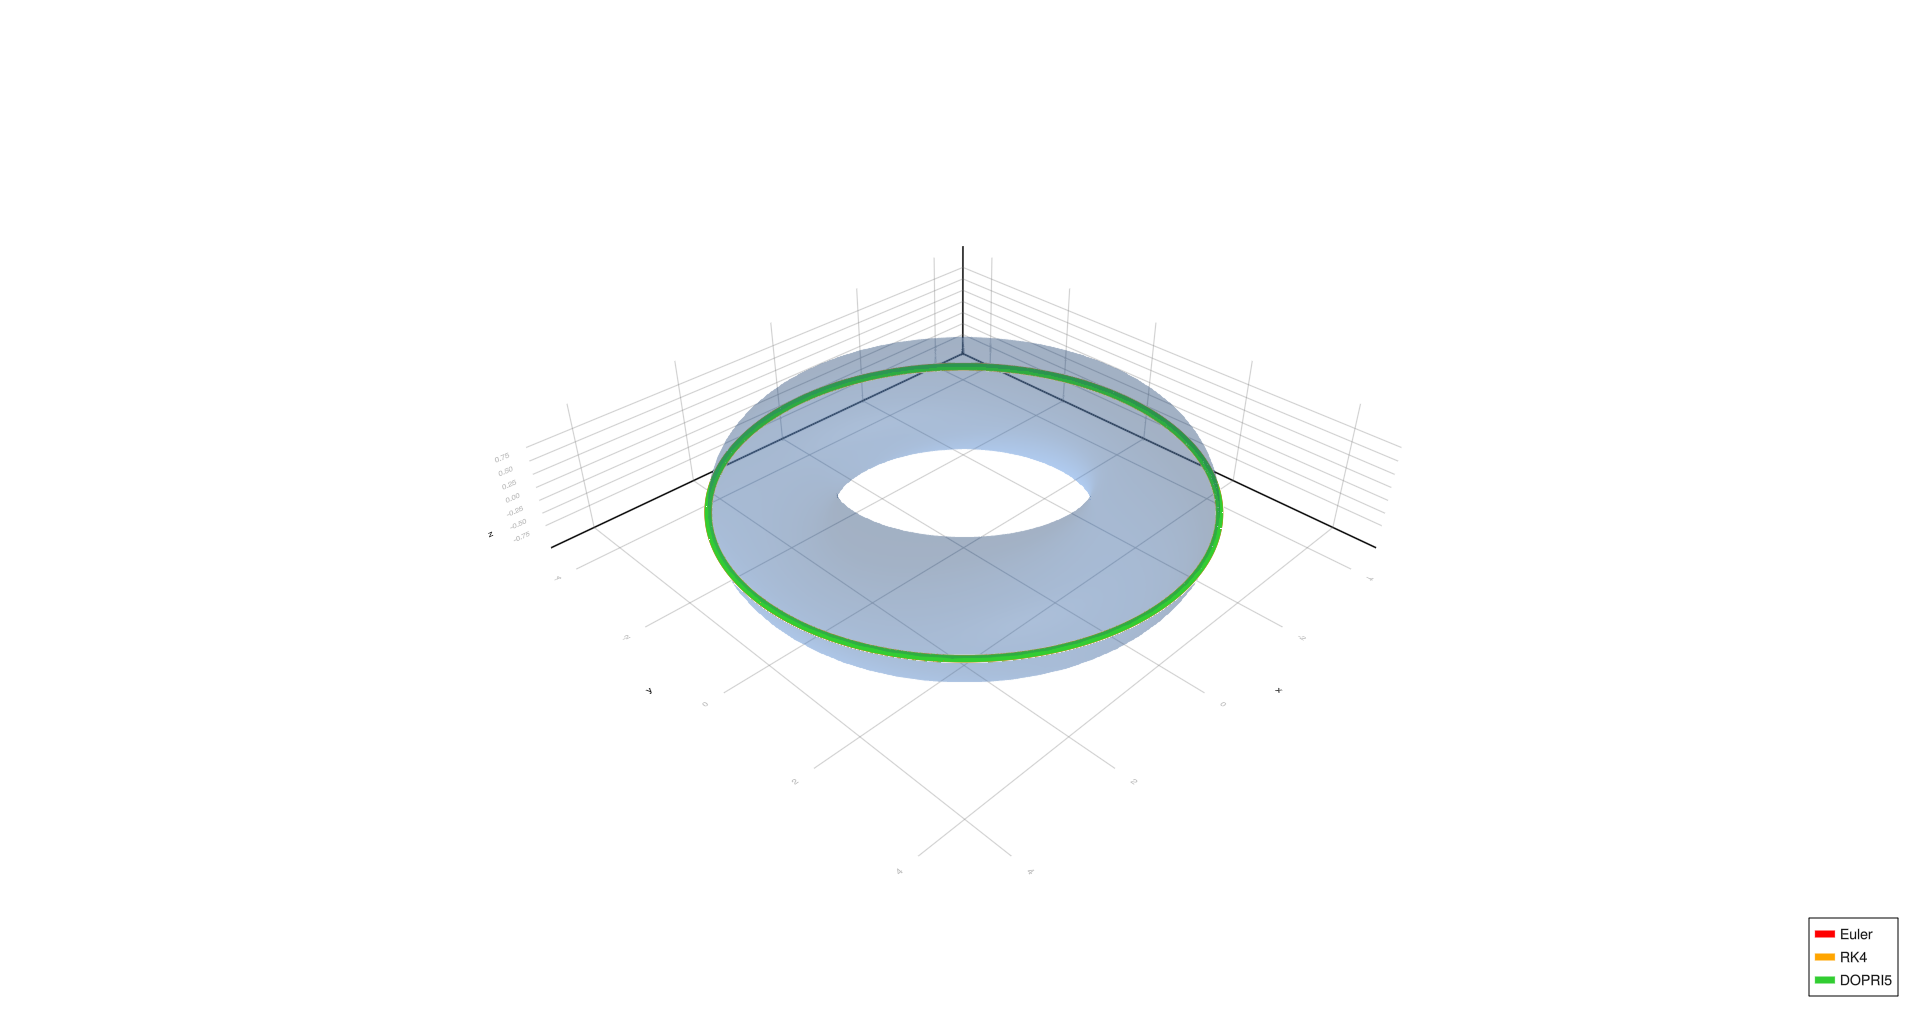
\includegraphics[width=\linewidth]{ou_eq_h0001.png}
			\caption{Outer equator, \(h=0.0001\)}
		\end{subfigure}
		
		\caption{Torus geodesics}
	\end{figure}
	
	\clearpage
	\begin{figure}[H]
		\centering
		\begin{subfigure}{1\textwidth}
			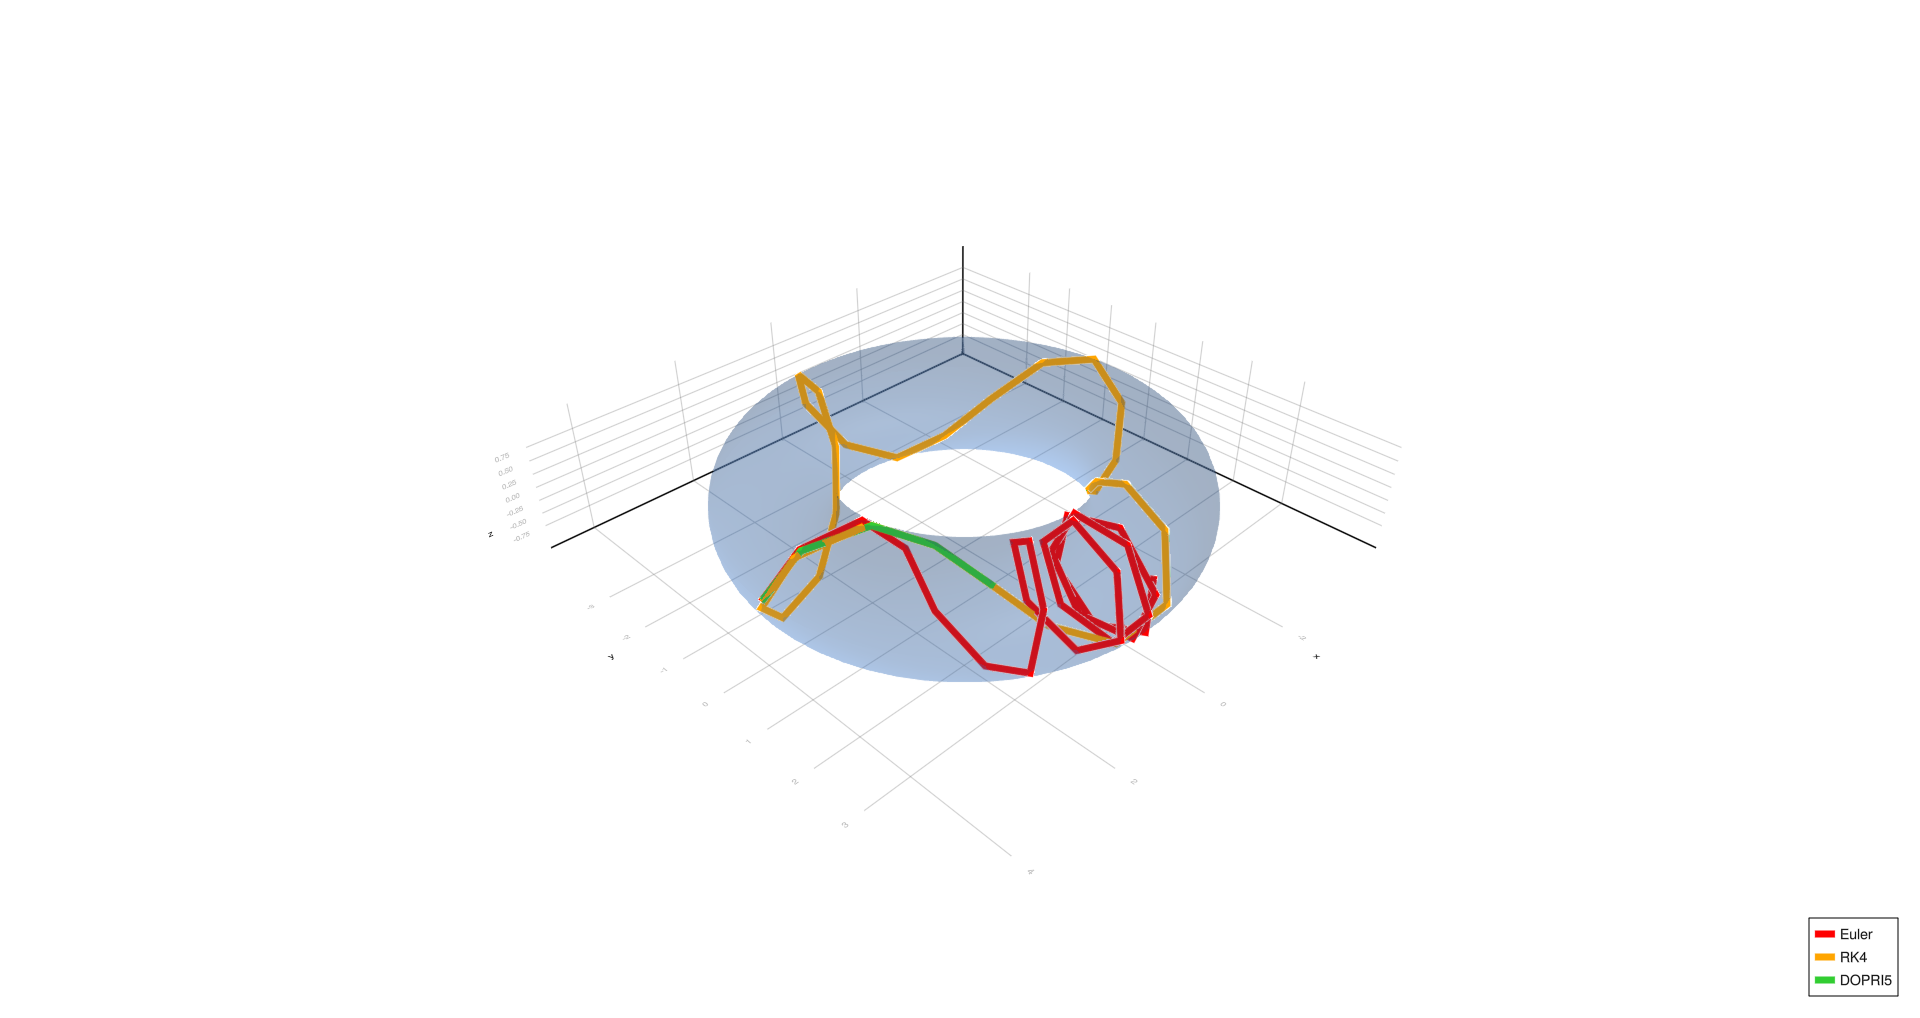
\includegraphics[width=\linewidth]{four_coils_h1.png}
			\caption{Four turns, \(h=1.0\)}
		\end{subfigure}
		
		\vspace{3em}
		
		\begin{subfigure}{1\textwidth}
			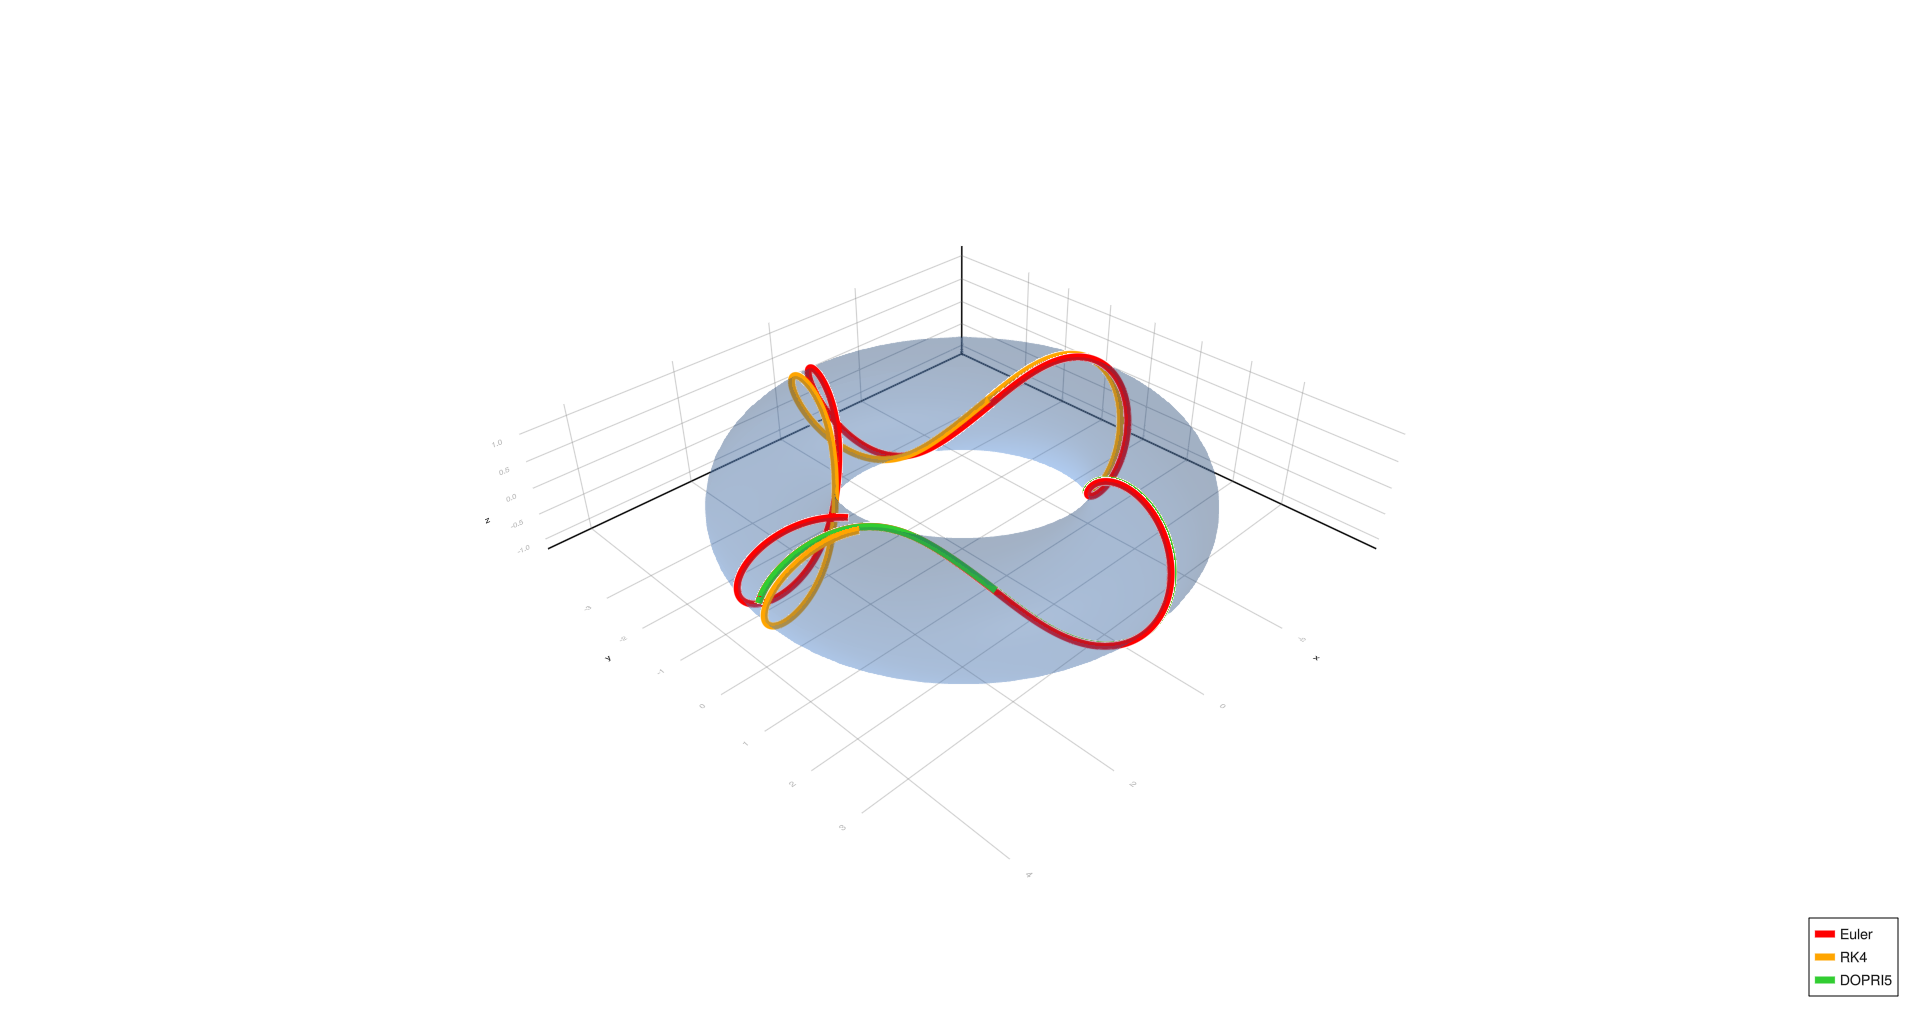
\includegraphics[width=\linewidth]{four_coils_h01.png}
			\caption{Four turns, \(h=0.01\)}
		\end{subfigure}
		
		\caption{Torus geodesics}
	\end{figure}
	
	\clearpage
	\begin{figure}[H]
		\centering
		\begin{subfigure}{1\textwidth}
			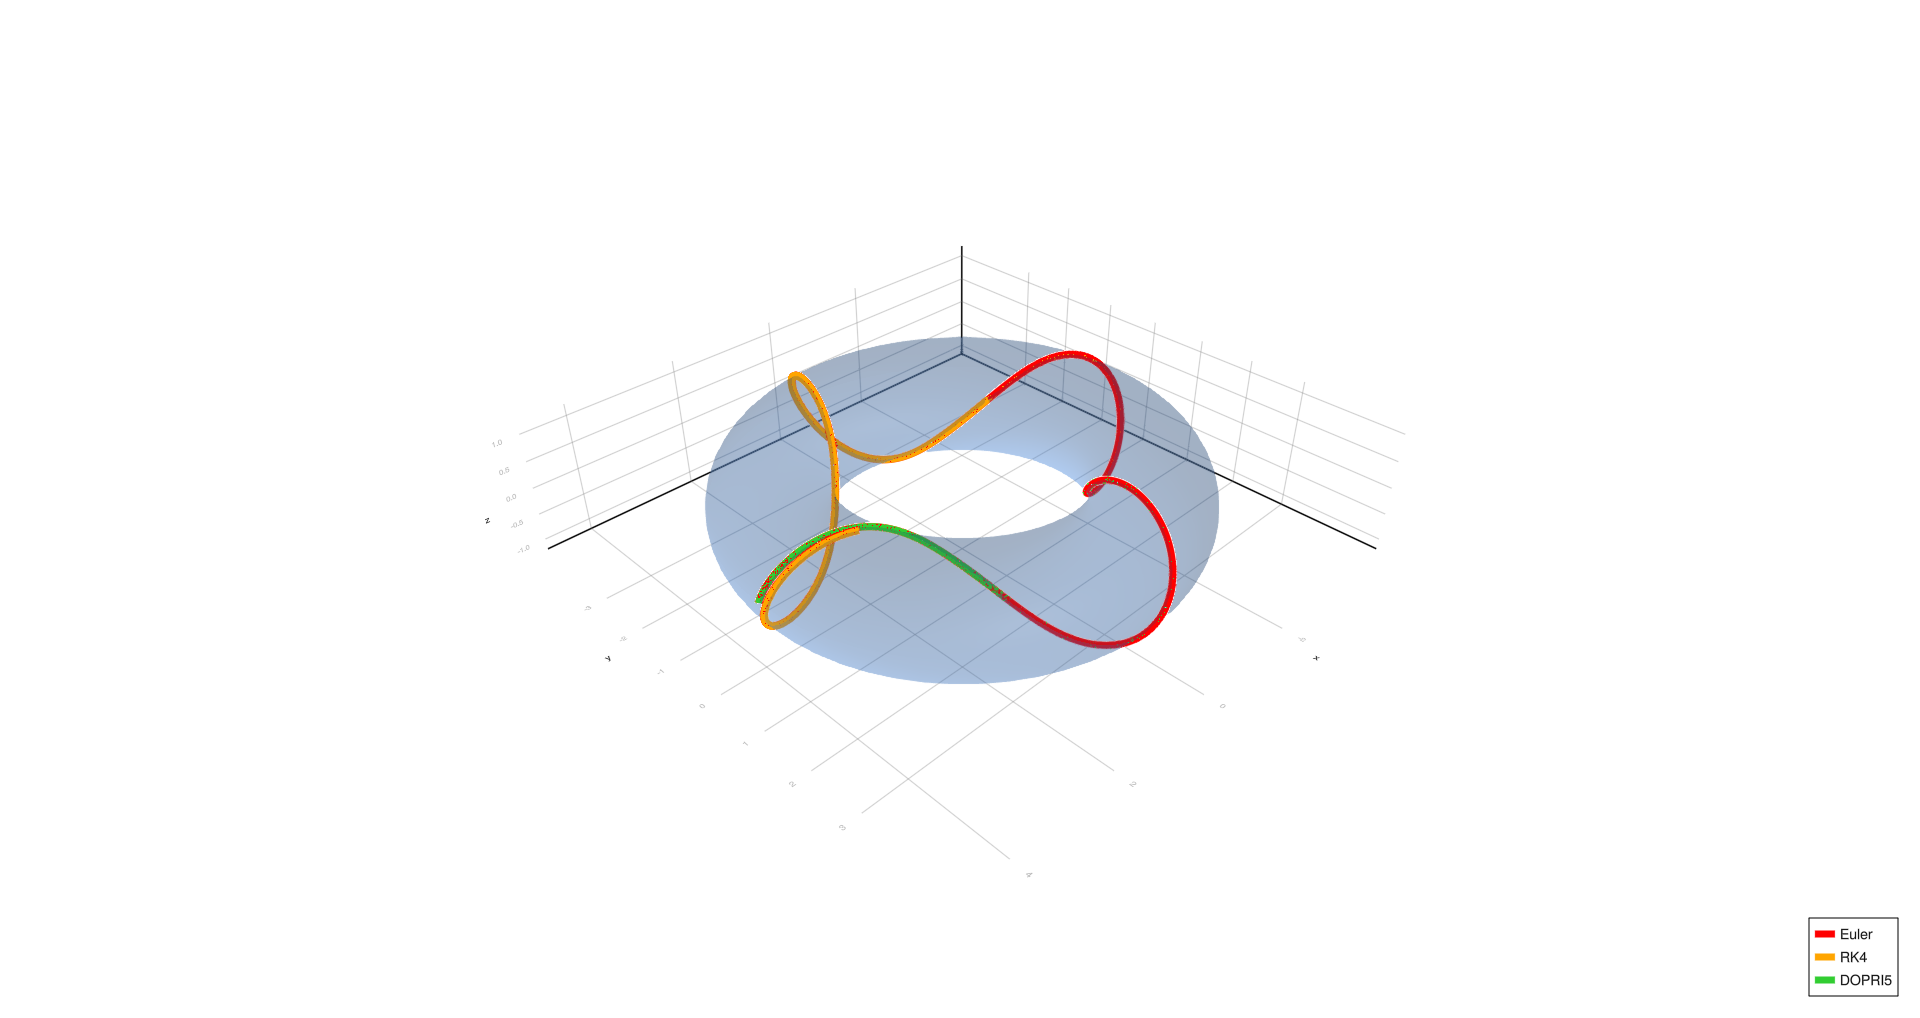
\includegraphics[width=\linewidth]{four_coils_h0001.png}
			\caption{Four turns, \(h=0.0001\)}
		\end{subfigure}
		
		\vspace{3em}
		
		\begin{subfigure}{1\textwidth}
			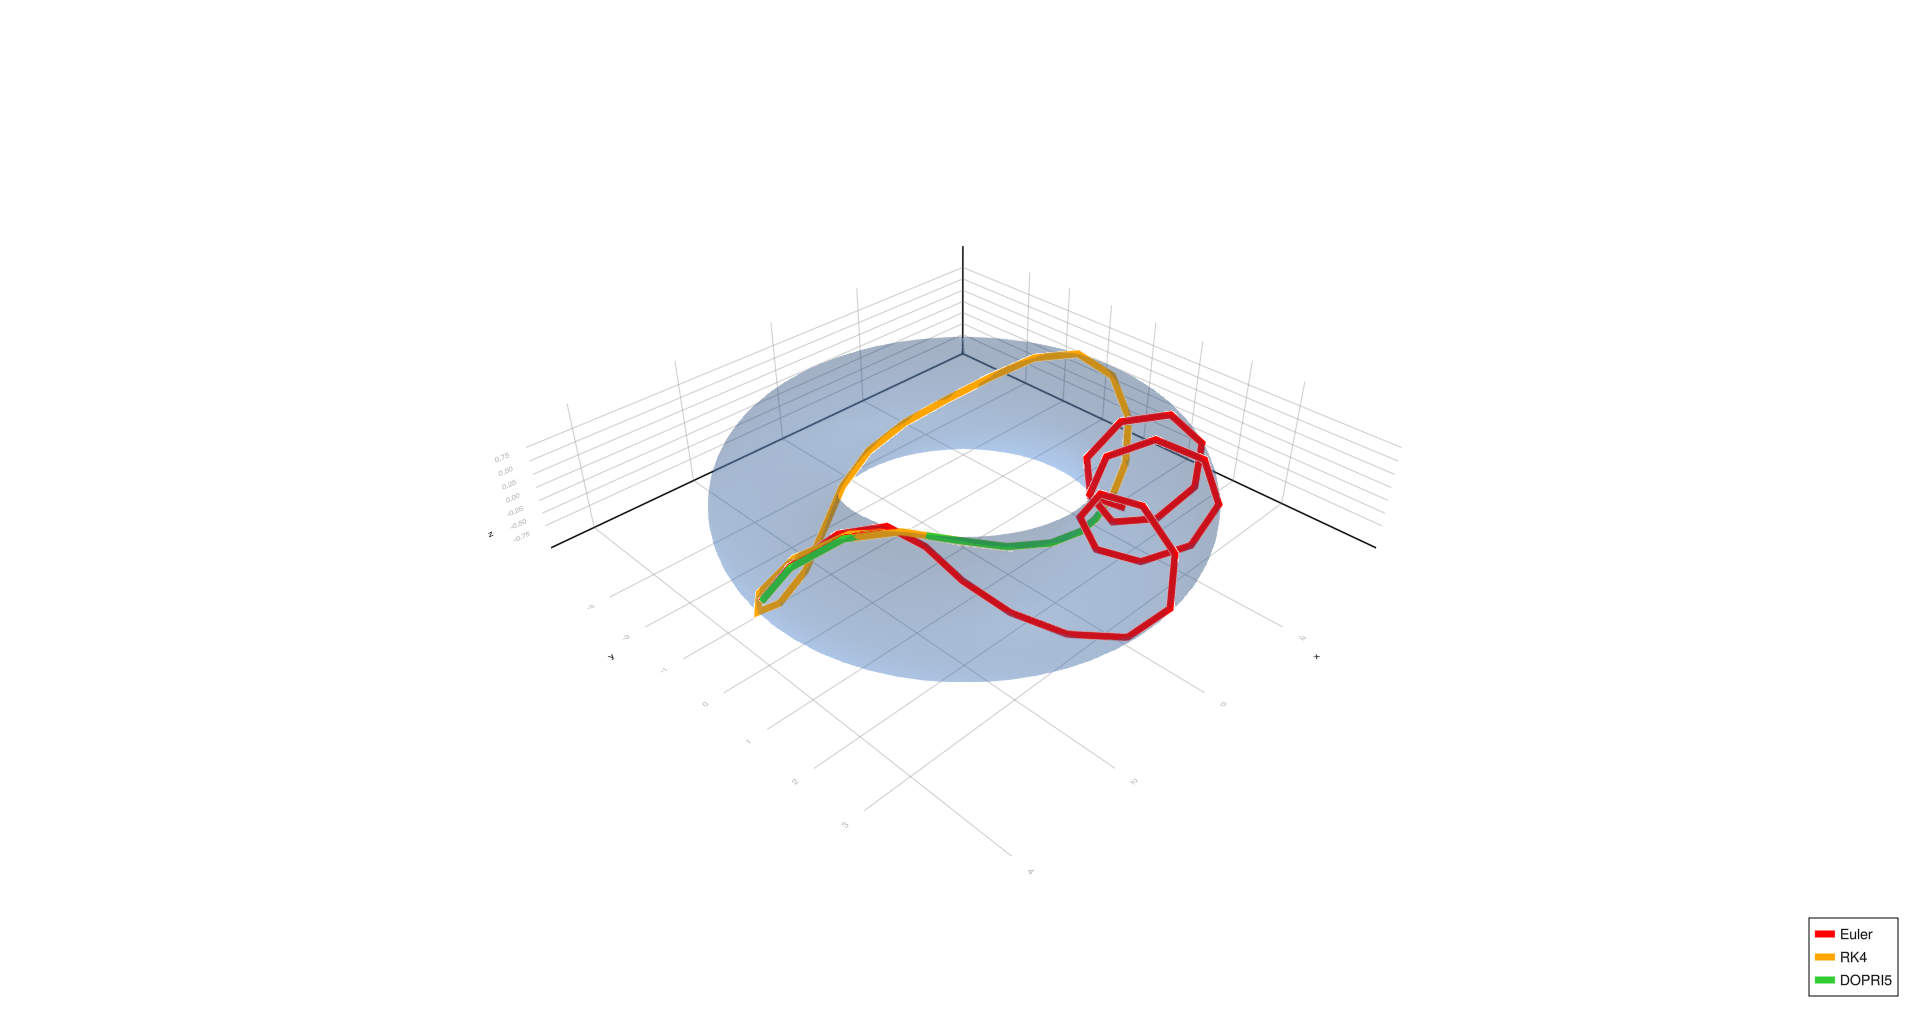
\includegraphics[width=\linewidth]{theone_h1.png}
			\caption{Complex spiral, \(h=1.0\)}
		\end{subfigure}
		
		\caption{Torus geodesics}
	\end{figure}
	
		\clearpage
	\begin{figure}[H]
		\centering
		\begin{subfigure}{1\textwidth}
			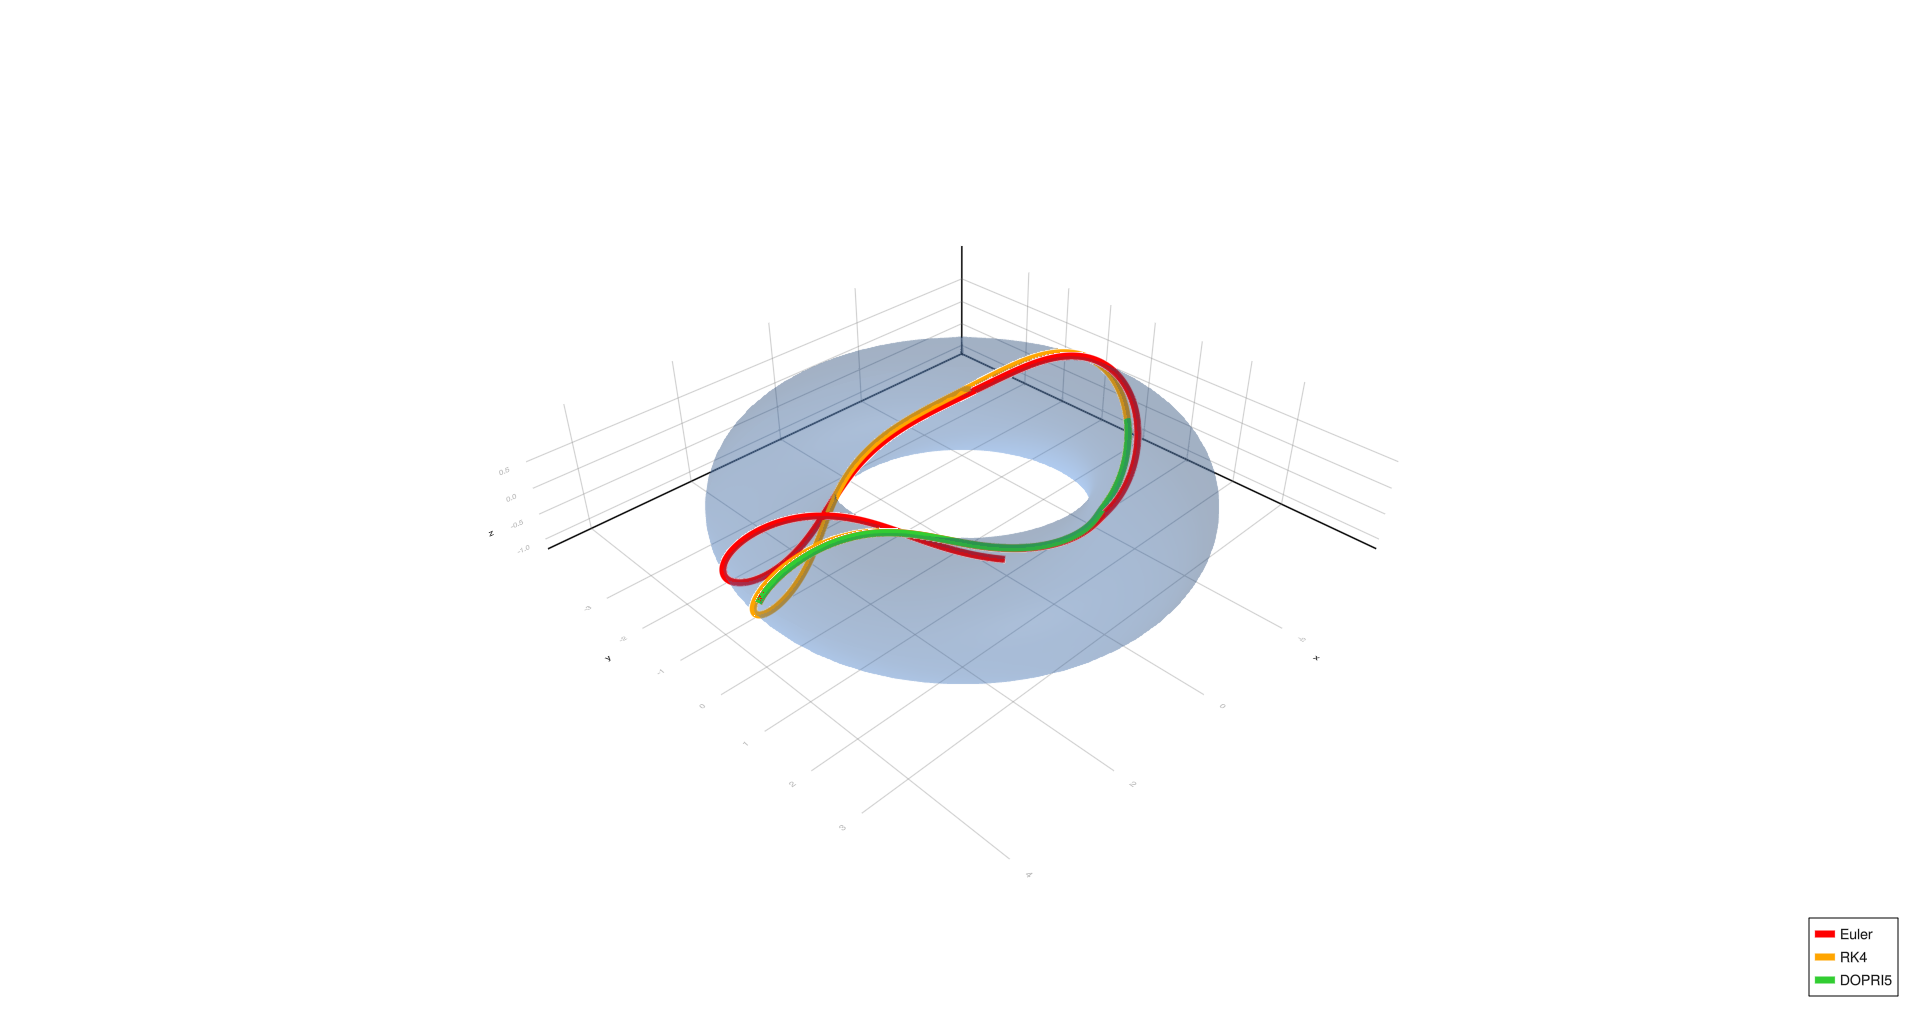
\includegraphics[width=\linewidth]{theone_h01.png}
			\caption{Complex spiral, \(h=0.01\)}
		\end{subfigure}
		
		\vspace{3em}
		
		\begin{subfigure}{1\textwidth}
			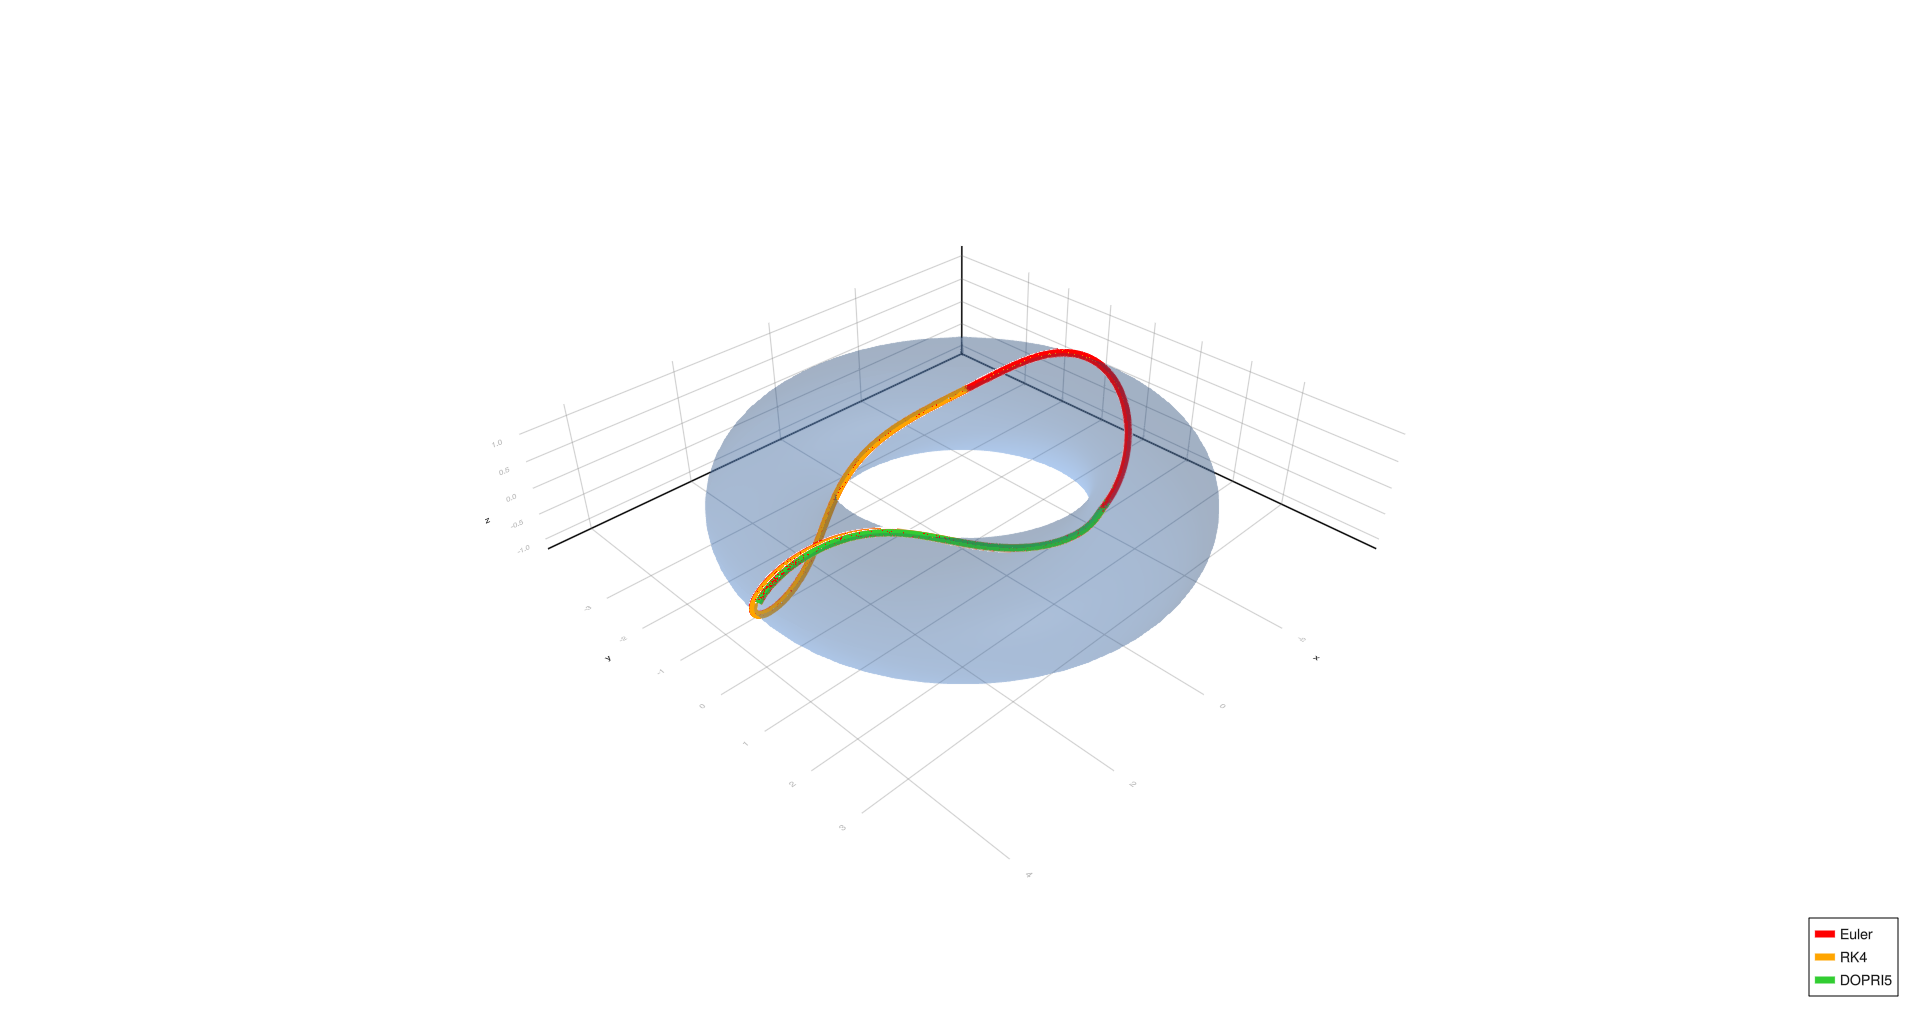
\includegraphics[width=\linewidth]{theone_h0001.png}
			\caption{Complex spiral, \(h=0.0001\)}
		\end{subfigure}
		
		\caption{Torus geodesics}
	\end{figure}
	
	\clearpage
	\begin{figure}[H]
		\centering
		\begin{subfigure}{1\textwidth}
			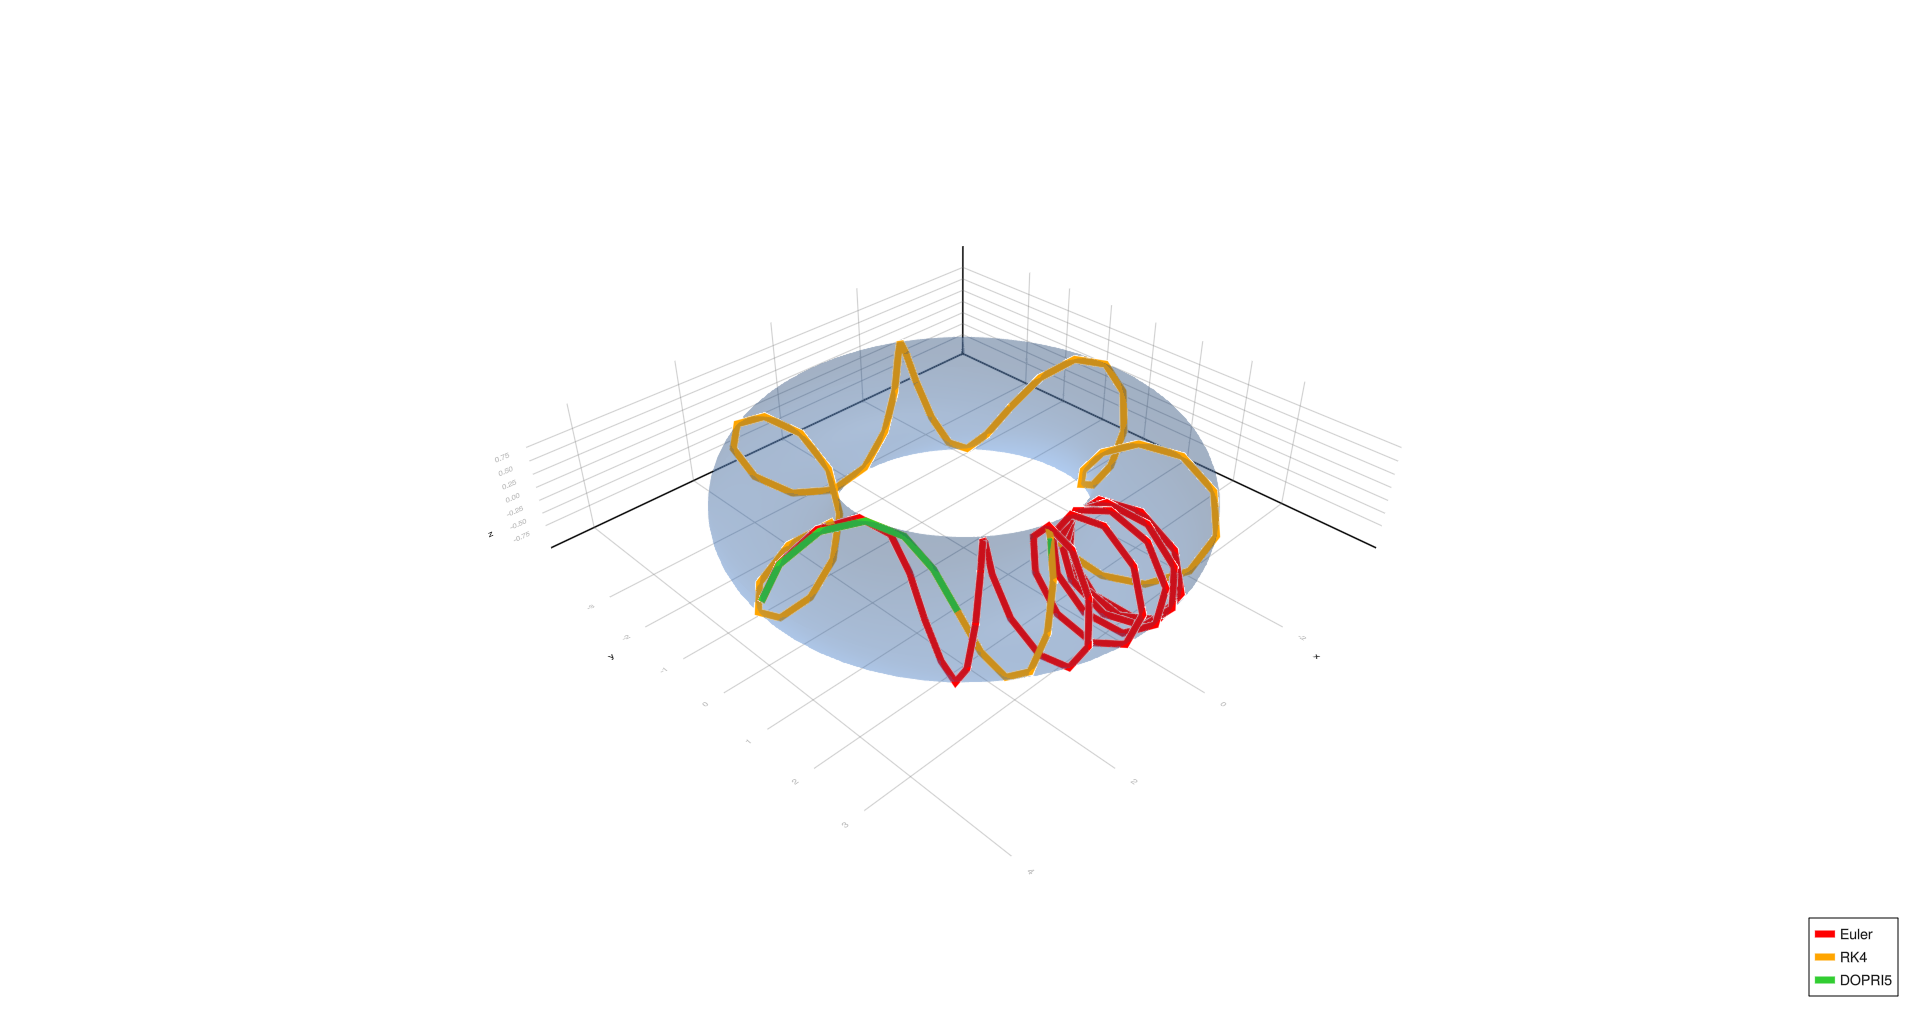
\includegraphics[width=\linewidth]{six_coils_h1.png}
			\caption{Six turns, \(h=1.0\)}
		\end{subfigure}
		
		\vspace{3em}
		
		\begin{subfigure}{1\textwidth}
			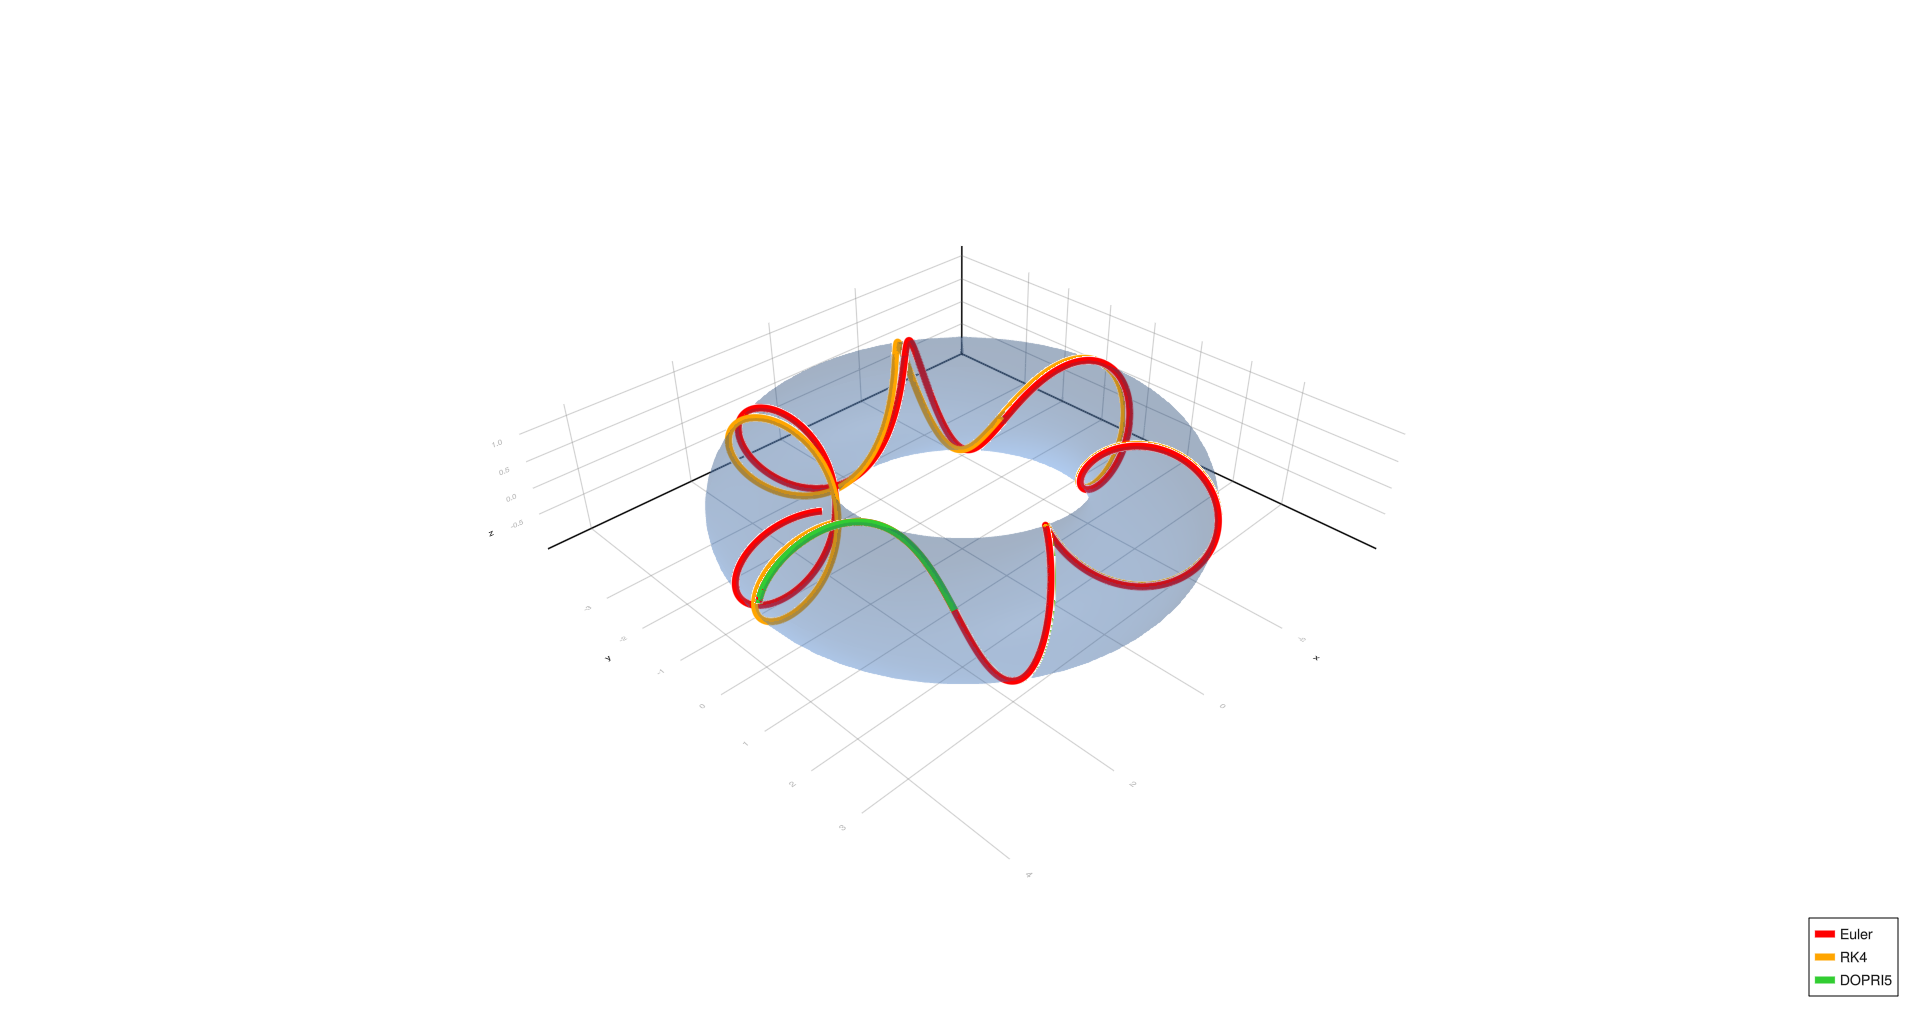
\includegraphics[width=\linewidth]{six_coils_h01.png}
			\caption{Six turns, \(h=0.01\)}
		\end{subfigure}
		
		\caption{Torus geodesics}
	\end{figure}
		\clearpage
		
	\begin{figure}[H]
		\centering
		\begin{subfigure}{1\textwidth}
			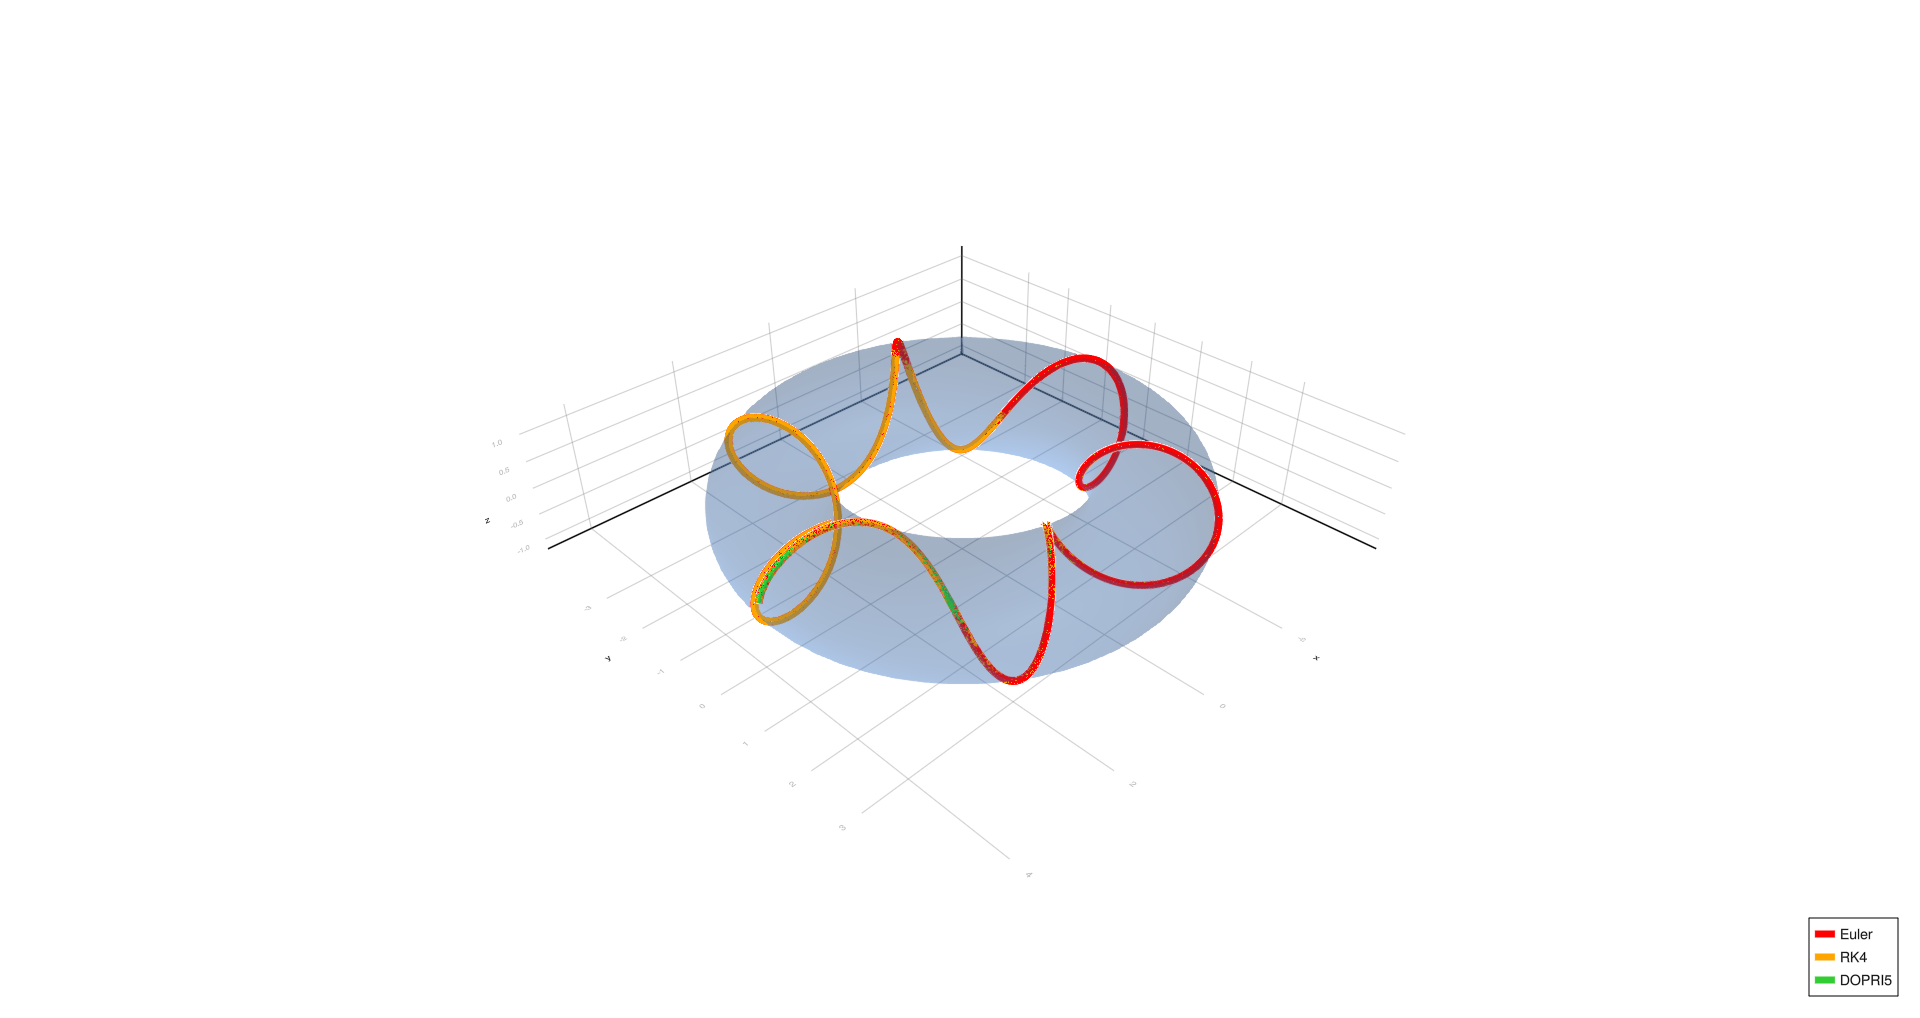
\includegraphics[width=\linewidth]{six_coils_h0001.png}
			\caption{Six turns, \(h=0.0001\)}
		\end{subfigure}
		
		\vspace{3em}
		
		\begin{subfigure}{1\textwidth}
			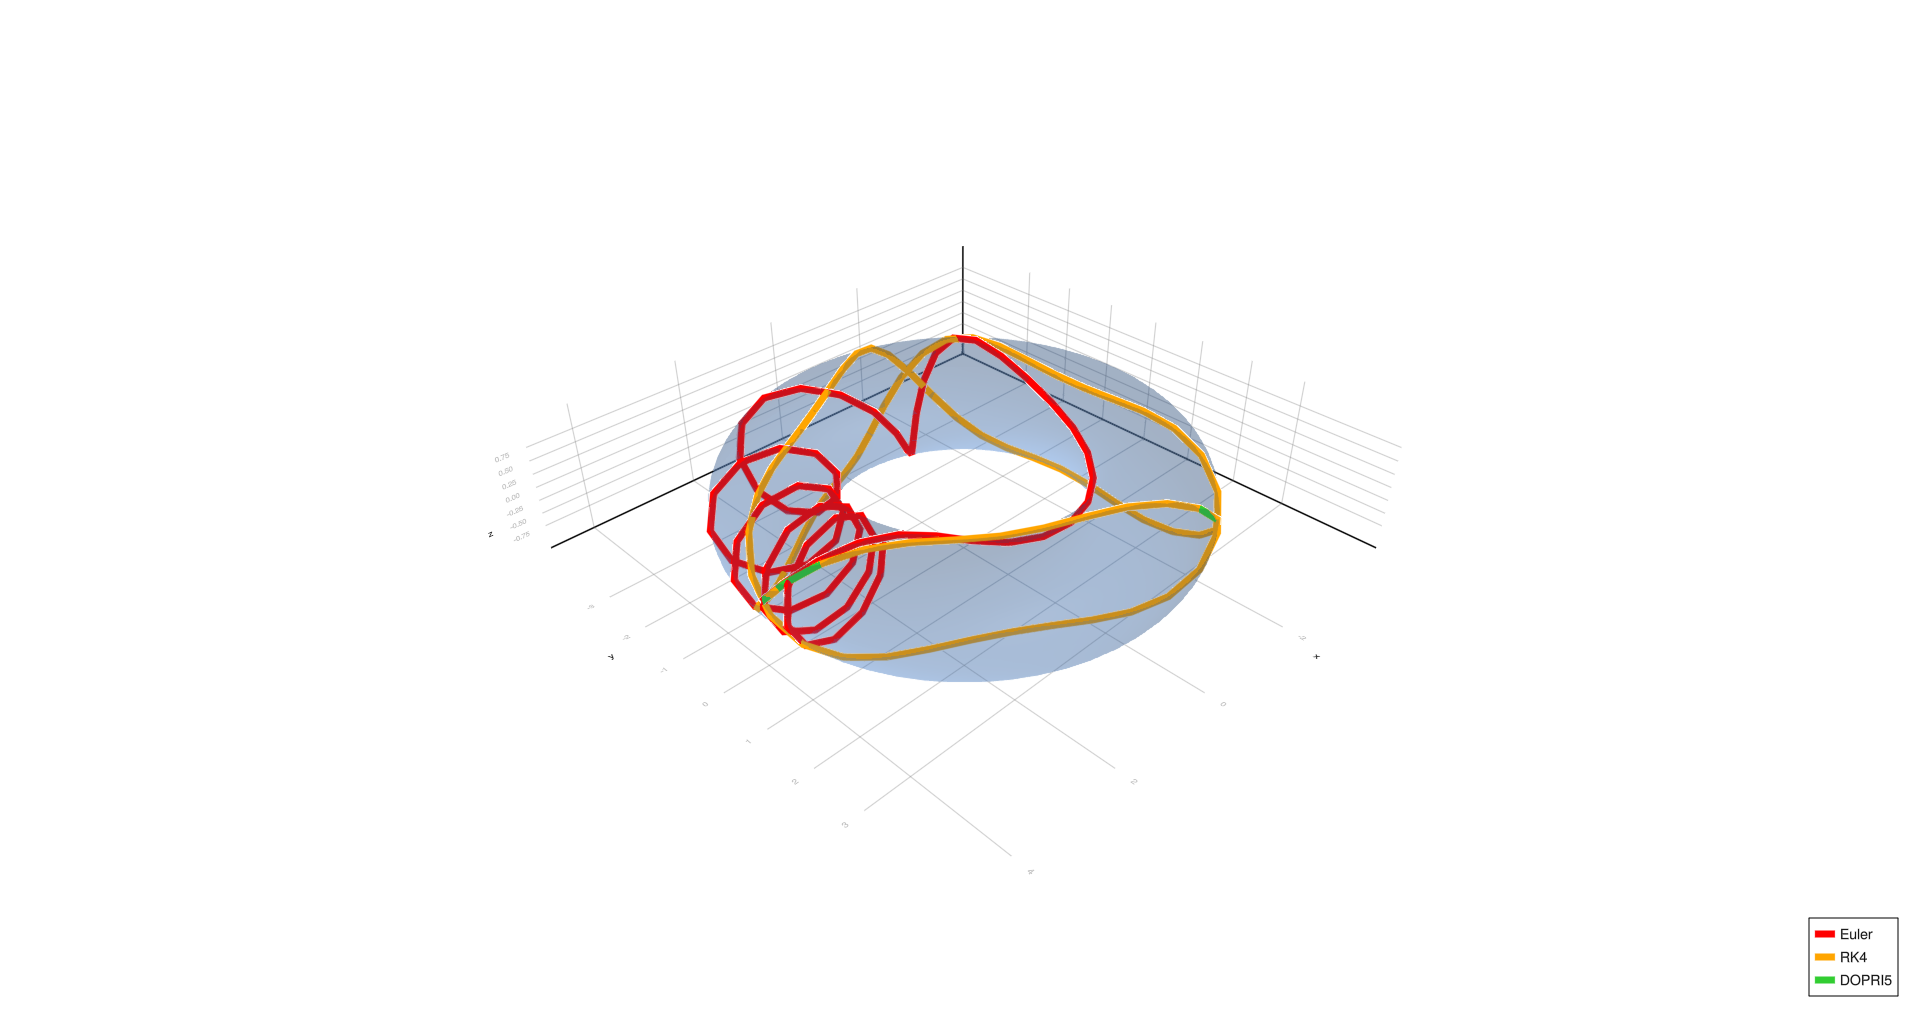
\includegraphics[width=\linewidth]{triangle_h1.png}
			\caption{Triangle, \(h=1.0\)}
		\end{subfigure}
		
		\caption{Torus geodesics}
	\end{figure}
	\clearpage
		\begin{figure}[H]
		\centering
		\begin{subfigure}{1\textwidth}
			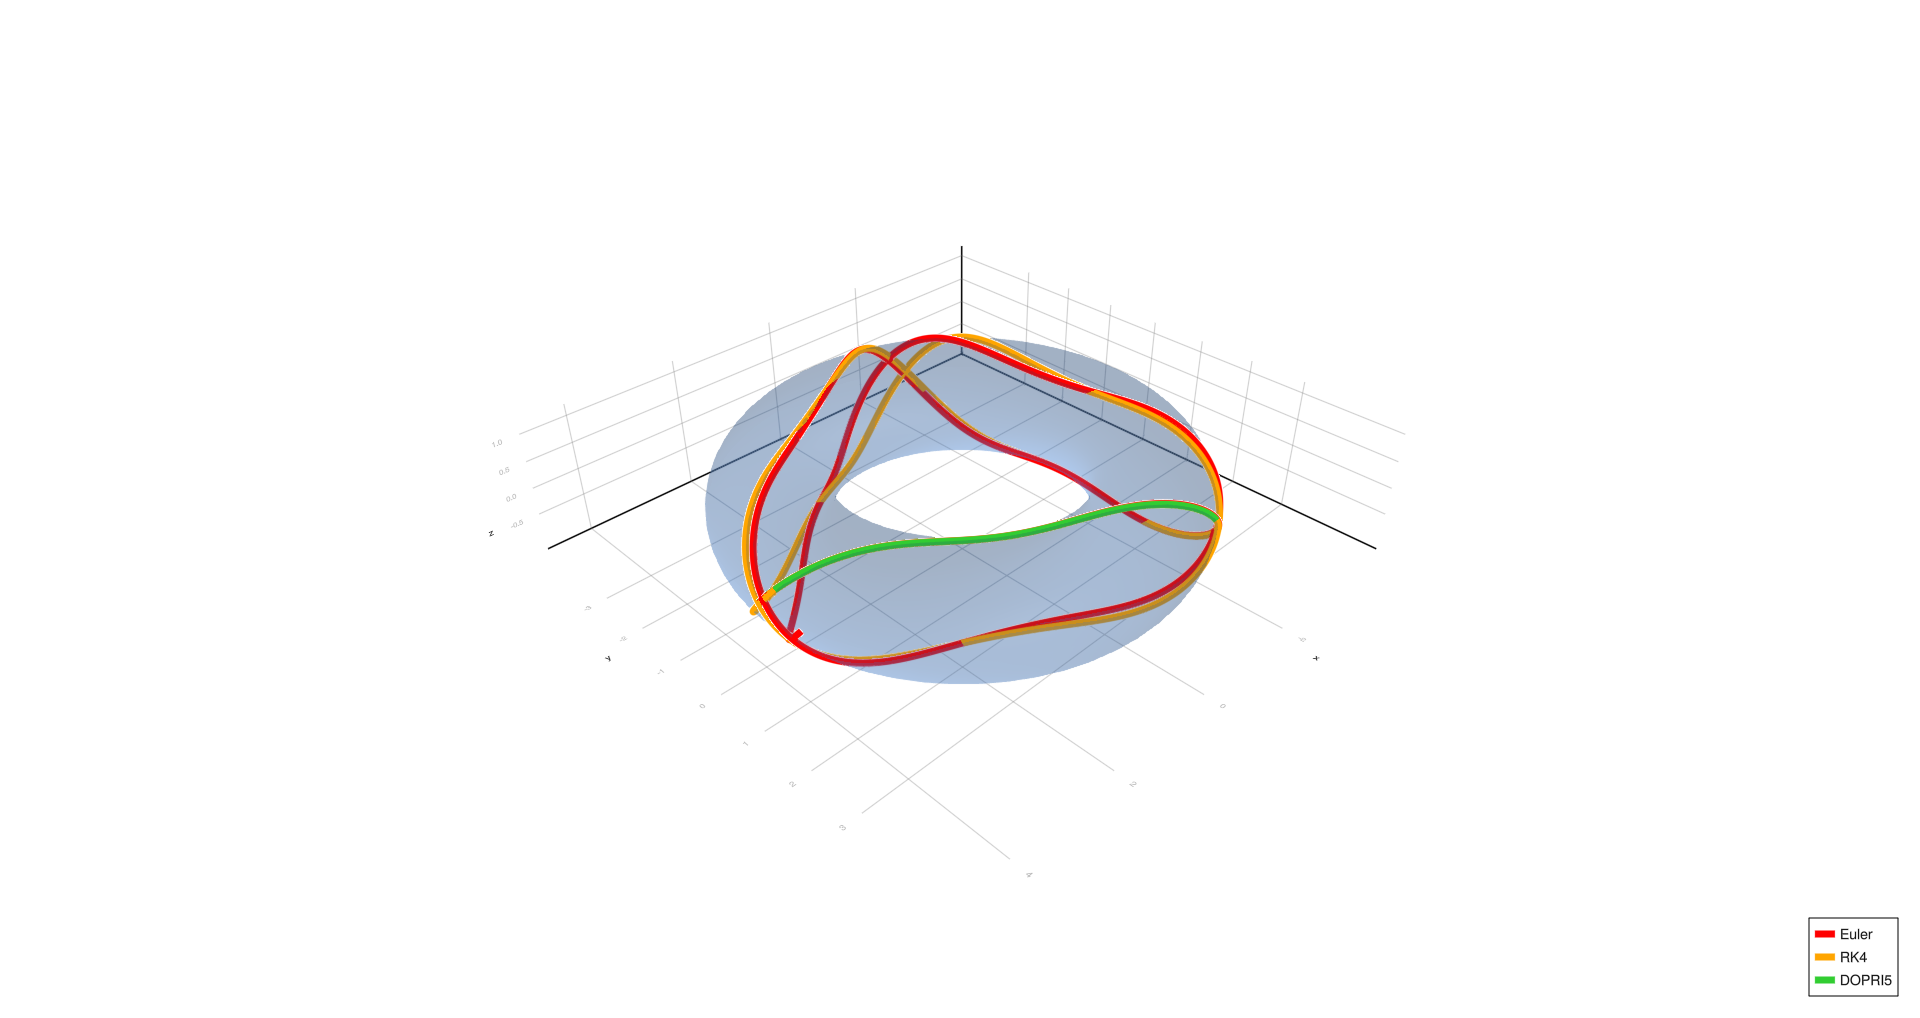
\includegraphics[width=\linewidth]{triangle_h01.png}
			\caption{Triangle, \(h=0.01\)}
		\end{subfigure}
		
		\vspace{3em}
		
		\begin{subfigure}{1\textwidth}
			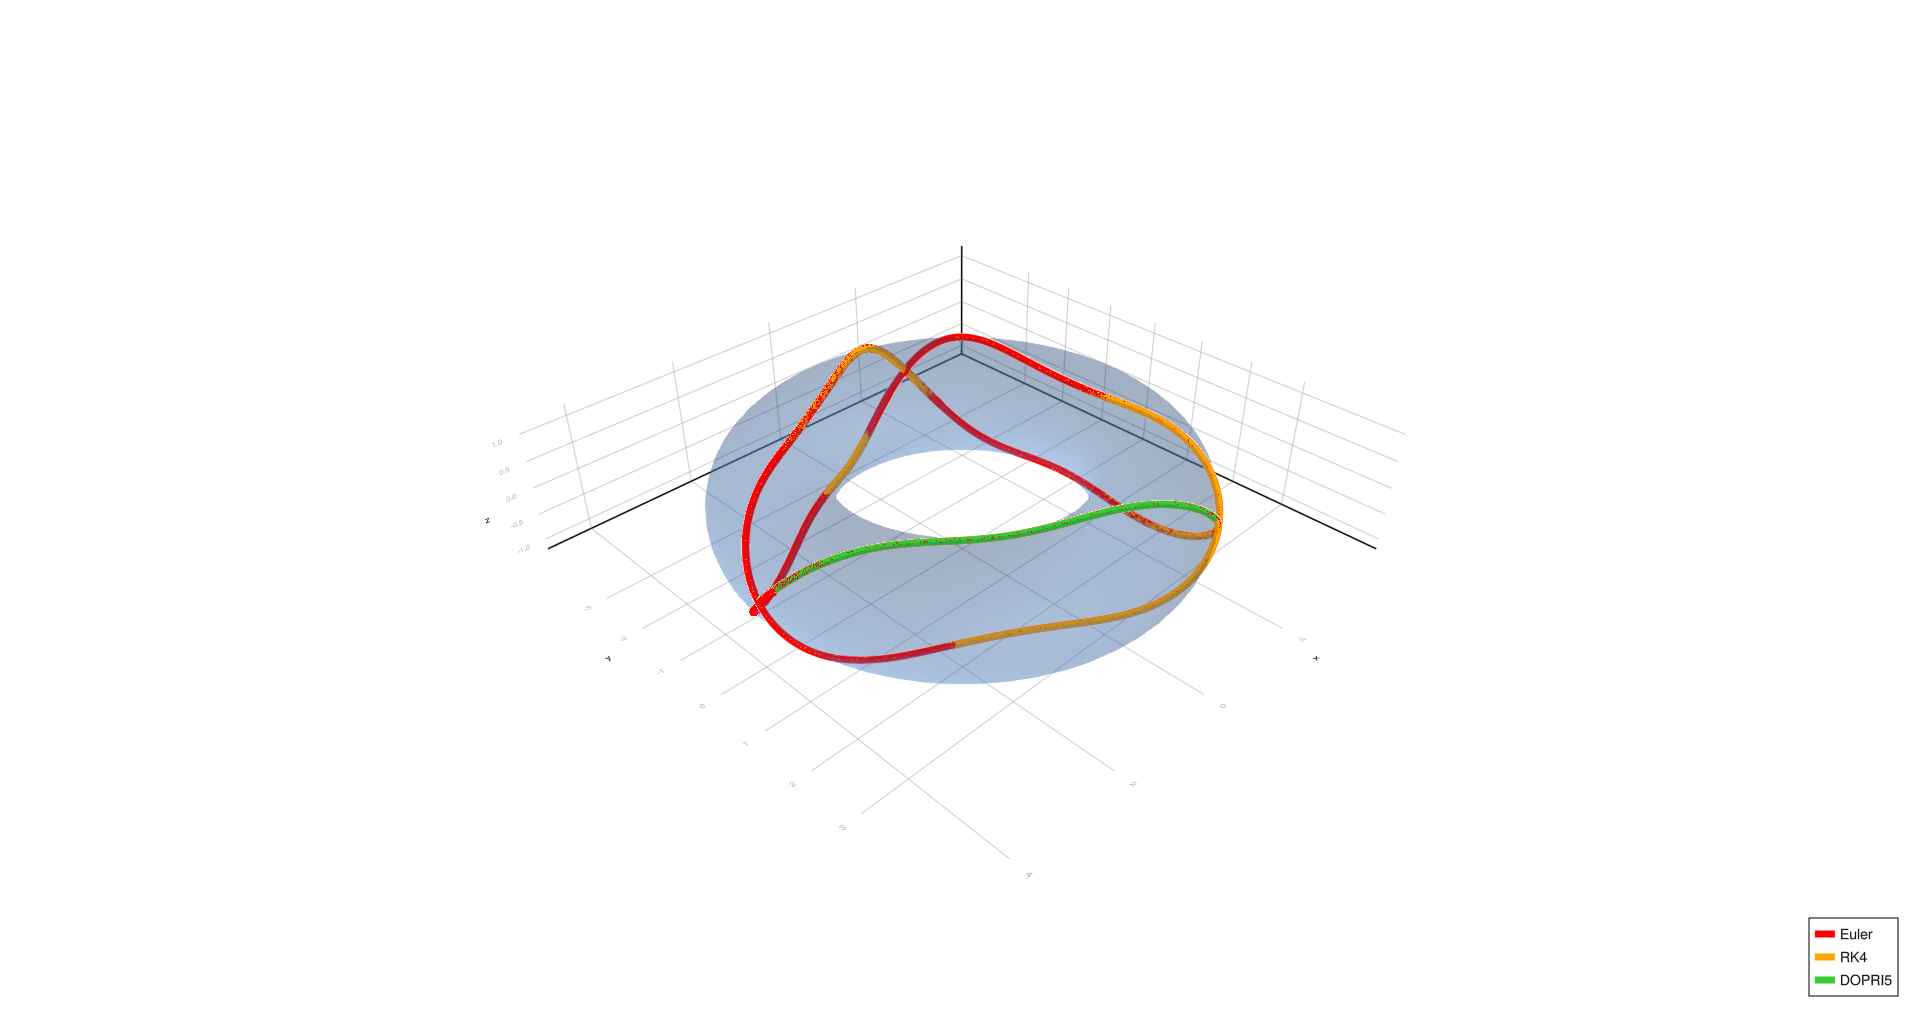
\includegraphics[width=\linewidth]{triangle_h0001.png}
			\caption{Triangle, \(h=0.0001\)}
		\end{subfigure}
		
		\caption{Torus geodesics}
	\end{figure}
	\clearpage

	\begin{figure}[H]
		\centering
		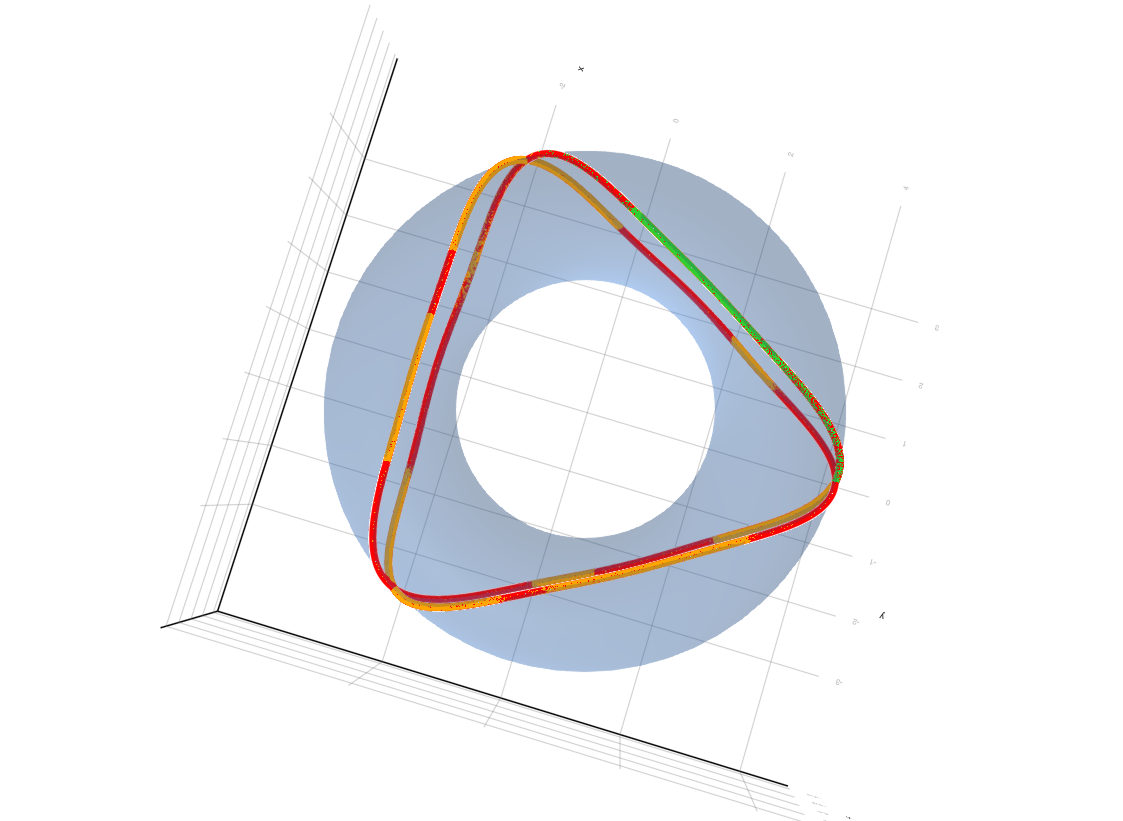
\includegraphics[width=1\textwidth]{triangle_uptop.png}
		\caption{Triangle, \(h=0.0001\) (from above)}
	\end{figure}
	\newpage
		
	\subsubsection{Empirical Observations}
	
	\begin{itemize}
		\item \textit{Inner and outer equators} remain stable across all step sizes and methods.
		\item \textit{Four turns, complex spiral, six turns, and triangle} show significant deviation with Euler at \(h = 1.0\), partial correction at \(h = 0.01\), and convergence with RK4/DOPRI5 at \(h = 0.0001\).
	\end{itemize}
	
	\subsubsection{Summary Table of Empirical Stability}
	
	\begin{table}[H]
		\centering
		\begin{tabular}{lccc}
			\toprule
			\textbf{Initial Condition} & \textbf{Step Size} & \textbf{Euler Accuracy} & \textbf{RK4 / DOPRI5 Accuracy} \\
			\midrule
			Inner Equator & 1.0 & Stable & Stable \\
			& 0.01 & Stable & Stable \\
			& 0.0001 & Stable & Stable \\
			\midrule
			Outer Equator & 1.0 & Stable & Stable \\
			& 0.01 & Stable & Stable \\
			& 0.0001 & Stable & Stable \\
			\midrule
			Four Turns & 1.0 & Large deviation & Stable \\
			& 0.01 & Minor deviation & Stable \\
			& 0.0001 & Stable & Stable \\
			\midrule
			Complex Spiral & 1.0 & Large deviation & Stable \\
			& 0.01 & Minor deviation & Stable \\
			& 0.0001 & Stable & Stable \\
			\midrule
			Six Turns & 1.0 & Large deviation & Stable \\
			& 0.01 & Minor deviation & Stable \\
			& 0.0001 & Stable & Stable \\
			\midrule
			Triangle & 1.0 & Large deviation & Stable \\
			& 0.01 & Minor deviation & Stable \\
			& 0.0001 & Stable & Stable \\
			\bottomrule
		\end{tabular}
		\caption{Empirical assessment of stability and accuracy of numerical methods for geodesics on the torus.}
	\end{table}
	\newpage
	\subsection{Conclusion}
	To compute geodesics accurately, higher-order methods such as Runge-Kutta 4 (RK4) and Dormand-Prince 5 (DOPRI5) are the most reliable. In our experiments, their results were nearly identical, with no practical difference in performance.
	\\\\
	While simpler methods like Euler's method can match the precision of higher-order methods in specific, uncomplicated cases, they are generally outperformed. However, reducing the step size significantly (e.g., to \(h = 0.0001\)) allows even Euler’s method to approach the accuracy of RK4 and DOPRI5.
	\\\\
	This presents a clear trade-off: Euler’s method is easy to implement but requires very small step sizes to achieve high accuracy, resulting in increased computational cost. Conversely, RK4 and DOPRI5 are more complex but provide stable and accurate results even with larger step sizes (e.g., \(h = 0.01\)), making them more efficient overall for most applications.

	
	
	\newpage
	\section{References}
	
	\begin{itemize}
		\item Kovač, Gregor. (2023). Sledenje žarku v neevklidskih prostorih. [Diplomsko delo, UL FRI]. Retrieved from \url{https://repozitorij.uni-lj.si/Dokument.php?id=172611&lang=slv}
		
		\item Dawkins, Paul. (2022). Section 2.9: Euler's Method [Article, Lamar University]. Retrieved from \url{https://tutorial.math.lamar.edu/classes/de/eulersmethod.aspx}
				
		\item eigenchris. (2018). Tensor Calculus 15: Geodesics and Christoffel Symbols (extrinsic geometry) [Video]. Retrieved from \url{https://www.youtube.com/watch?v=1CuTNveXJRc}
		
		
		\item Irons, Mark Lawrence. (2005). The Geodesics of the Torus [Article]. Retrieved from \url{http://www.rdrop.com/~half/math/torus/geodesics.xhtml}
		
		\item Vas, Lia. (n.d.). Differential Geometry Handouts. [PDF files, Dept. of Mathematics, Saint Joseph's University]. Retrieved from \url{https://liavas.net/courses/math430/}
	\end{itemize}
	
	
\end{document}



